\documentclass[a4paper]{article}

\usepackage[utf8]{inputenc}
\usepackage[a4paper,margin=3cm]{geometry}
%\usepackage[symbol]{footmisc}
\renewcommand*{\thefootnote}{\fnsymbol{footnote}} % footnotes

\usepackage{booktabs}
\usepackage{caption}
\usepackage{subcaption}
\usepackage{multirow}
\usepackage{geometry}

\usepackage{graphicx}
\usepackage[dvipsnames]{xcolor}
\usepackage{tikz}
\usepackage{pgfplots}
\usepackage{comment}

\usepackage{amsmath, amsfonts}
\usepackage{amssymb}
\usepackage{physics}

\usepackage{bm}
\usepackage{listings}

\usepackage{hyperref}
\hypersetup{
	colorlinks=true,
	urlcolor=tabblue,
	linkcolor=tabblue,
	citecolor=tabgreen
}

\usepackage[citestyle=numeric-comp]{biblatex}

%%%%%%% TIKZ OPTIONS FOR PGFPLOTSX
\usetikzlibrary{arrows.meta}
\usetikzlibrary{backgrounds}
\usetikzlibrary{decorations.markings}
\usetikzlibrary{patterns}
\pgfplotsset{compat=newest}
\usepgfplotslibrary{patchplots}
\usepgfplotslibrary{fillbetween}
\pgfplotsset{%
    layers/standard/.define layer set={%
        background,axis background,axis grid,axis ticks,axis lines,axis tick labels,pre main,main,axis descriptions,axis foreground%
    }{
        grid style={/pgfplots/on layer=axis grid},%
        tick style={/pgfplots/on layer=axis ticks},%
        axis line style={/pgfplots/on layer=axis lines},%
        label style={/pgfplots/on layer=axis descriptions},%
        legend style={/pgfplots/on layer=axis descriptions},%
        title style={/pgfplots/on layer=axis descriptions},%
        colorbar style={/pgfplots/on layer=axis descriptions},%
        ticklabel style={/pgfplots/on layer=axis tick labels},%
        axis background@ style={/pgfplots/on layer=axis background},%
        3d box foreground style={/pgfplots/on layer=axis foreground},%
    },
}

\newcommand{\beq}{\begin{equation}}
\newcommand{\eeq}{\end{equation}}
\newcommand{\sgn}{\mathrm{sgn}}

\newcommand{\red}[1]{\color{red}{#1}}

\newcommand{\mref}{{\color{red}0.0}} % missing ref
\newcommand{\todo}{\noindent{\color{tabred}[To be continued\dots]}}

\definecolor{tabred}{RGB}{214, 39, 40}
\definecolor{tabblue}{HTML}{1f77b4}
\definecolor{tabgreen}{HTML}{2ca02c}

%\usepackage[usenames,dvipsnames]{color} % more flexible names for syntax highlighting colors

\lstset{
    basicstyle=\ttfamily, 
    numbers=left, 
    numberstyle=\small\ttfamily\color{ForestGreen},
    stepnumber=1,              
    numbersep=10pt, 
    numberfirstline=true, 
    numberblanklines=true, 
    tabsize=4,
    lineskip=0pt,
    aboveskip=10pt,
    belowskip=10pt,
    extendedchars=true,
    breaklines=true,
    %backgroundcolor=\color{ForestGreen!10},
    keywordstyle=\color{blue}\bfseries,
    identifierstyle=, % using emph or index keywords
    commentstyle=\color{ForestGreen},
    stringstyle=\color{Maroon},
    showstringspaces=false,
    showtabs=false,
    upquote=false,
    texcl=true % interpet comments as LaTeX
}

\lstdefinelanguage{julia}
{
  keywordsprefix=\@,
  morekeywords={
    exit,whos,edit,load,is,isa,isequal,typeof,tuple,ntuple,uid,hash,finalizer,convert,promote,
    subtype,typemin,typemax,realmin,realmax,sizeof,eps,promote_type,method_exists,applicable,
    invoke,dlopen,dlsym,system,error,throw,assert,new,Inf,Nan,pi,im,begin,while,for,in,return,
    break,continue,macro,quote,let,if,elseif,else,try,catch,end,bitstype,ccall,do,using,module,
    import,export,importall,baremodule,immutable,local,global,const,Bool,Int,Int8,Int16,Int32,
    Int64,Uint,Uint8,Uint16,Uint32,Uint64,Float32,Float64,Complex64,Complex128,Any,Nothing,None,MPO,MPS,
    function,type,typealias,abstract
  },
  sensitive=true,
  morecomment=[l]{\#},
  morestring=[b]',
  morestring=[b]" 
}


\addbibresource{misc/bibliography.bib}

\begin{document}

\begin{center}
    {\bfseries {\Large Finite-size DMRG characterization of the}} \\[0.8em]
    {\bfseries {\Large 1D Fermi-Hubbard model phase diagram}}\\[0.8em]
    {\bfseries {\Large under bosonization framework}} \\[1em]
    \large University of Pisa, a.y.~2024-2025 \\[0.8em]
    Alessandro Gori\footnote{\href{mailto:a.gori23@studenti.unipi.it}{a.gori23@studenti.unipi.it} / \href{https://github.com/nepero27178}{nepero27178@github.com}} \\[0.8em]
    \scriptsize Final project for the Master's Degree course ``Quantum Liquids''
    
\end{center}

\renewcommand*{\thefootnote}{\arabic{footnote}}
\setcounter{footnote}{0}

\begin{abstract}
    The one-dimensional Fermi-Hubbard model at zero temperature is studied, employing finite-size DMRG algorithm to investigate some of its ground state properties. The model contains a hopping term between neighbouring sites, a finite on-site interaction energy, and a chemical potential. In order to investigate the zero-temperature ground-state properties of the model, finite-size DMRG was used. 
    
    The entire project heavily relies upon the precedent project carried out by the author together with Marco Pompili, where the 1D Bose-Hubbard model was studied using finite-size DMRG. You may find \href{https://github.com/mrc-pop/BoseHubbardDMRG}{at this link} our previous work.\\
    \begin{center}
        {\footnotesize All of the code can be found at open-access in \href{https://github.com/nepero27178/FermiHubbardDMRG}{this repository}:\\ \url{https://github.com/nepero27178/FermiHubbardDMRG}}
    \end{center}
\end{abstract}
\tableofcontents

\clearpage

\section{Theoretical introduction to bosonization}

This first, vast section is devoted to the introduction of an extremely powerful technique in one-dimensional fermionic problems, namely, bosonization. It is widely based on the comprehensive work of \citeauthor{giamarchi2003quantum}, \cite{giamarchi2003quantum}. I won't get deep in the calculations neither in refined points about the method, being this last arbitrarily vast. The first part of this section deals with the spinless (a.k.a. polarized) case; the second part introduces the spin degree of freedom.

\subsection{Bosonization in a nutshell for spinless fermions}

\begin{figure}
	\centering
	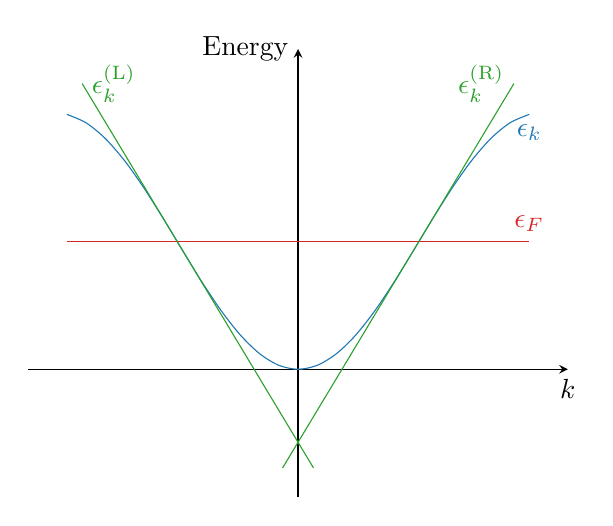
\begin{tikzpicture}
	\begin{axis}[
			axis lines=center,
			xlabel={$k$},
			ylabel={Energy},
			xlabel style={below},
			ylabel style={left},
			xtick=\empty,
			ytick=\empty,
			xmin=-3.5, xmax=3.5,
			ymin=-1.0, ymax=2.5
		]
		\addplot[domain=-3:3, smooth, color=tabblue]
			{1-cos(deg(x))} node[below] {$\epsilon_k$};
		
		\addplot[domain=-3:3, color=tabred]
			{1} node[above] {$\epsilon_F$};
			
		\addplot[domain=0.2:-2.8, color=tabgreen]
			{-0.57-x} node[right] {$\epsilon_k^{(\mathrm L)}$};
		
		\addplot[domain=-0.2:2.8, color=tabgreen]
			{-0.57+x} node[left] {$\epsilon_k^{(\mathrm R)}$};
	\end{axis}
\end{tikzpicture}
	\caption{Sketch of the fermionic band $\epsilon_k$, the Fermi level $\epsilon_F$ and the two linear bands $\epsilon_k^{(\mathrm{L}/\mathrm{R})}$ used to approximate the original bands around the Fermi surface. The double-linear model is often referred to as the Tomonaga-Luttinger model.}
	\label{fig:bands}
\end{figure}

The key idea is simple: start from a conventional fermionic-metallic hamiltonian,
\[
	\hat H = \hat H_0 + \hat V = \sum_k \xi_k \hat c_k^\dagger \hat c_k + \hat V
\]
(I will leave the interaction unspecified, for a moment) where $\xi_k = \epsilon_k - \epsilon_F$ and I am using spinless fermions, for normal bands in ordinary fillings.
Consider Fig.~\ref{fig:bands}: the approximation in the above equation is exactly given by making the following assumption: since at low temperature (which, in metals, is a very broad definition) all the relevant Physics takes place at $\xi \sim 0$, and both the deep-down/far-away single-particle states do not contribute either due to Pauli pressure or state depletion, one can as well study the model:
\[
	\epsilon_k \to \left\{\epsilon_k^{(\mathrm L)}, \epsilon_k^{(\mathrm R)} \right\}
\]
Let $s$ be the side index, $s \in \left\{\mathrm L, \mathrm R\right\}$, with
\[
\sgn(s) = \begin{cases}
	+1 \quad \text{if} \quad s = \mathrm R \\
	-1 \quad \text{if} \quad s = \mathrm L
\end{cases}
\]
Then I may approximate around the Fermi surface (in one dimension degenerated in two points)
\[
	\hat H_0 \simeq \hat K_0 \equiv \sum_{s \in \left\{\mathrm L, \mathrm R\right\}} \sum_k \hbar v_F \left( \sgn(s) k -  k_F \right) \left[ \hat c_k^{(s)} \right]^\dagger \hat c_k^{(s)}
\]
being $k_F \equiv \sqrt{2m\epsilon_F/\hbar}$ the Fermi wavevector and $v_F \equiv \hbar k_F / m$. $\hat K_0$ is the Tomonaga-Luttinger model. In the following, I will set $\hbar=1$. Now, consider the side-wise density operators,
\[
	\hat \rho_q^{(s)} \equiv \sum_k  \left[ \hat c_{k+q}^{(s)} \right]^\dagger \hat c_k^{(s)}
\]
Let me use a slightly different, somewhat lighter notation:
\[
	\hat \rho_q^{(s)} \leftrightarrow \hat \rho_s (q)
\]
From now on, I will proceed only highlighting the important result in the bosonization procedure, since all the detailed derivation is included in \cite{giamarchi2003quantum}.

\subsubsection{Boson operators}

The pivotal result in the bosonization technique is the following:
\beq\label{eq:density-commutator}
	\comm{\hat \rho_s (q)}{\hat \rho_{s'} (-q')} = - \delta_{ss'} \delta_{qq'} \sgn(s) \frac{qL}{2\pi}
\eeq
where $L$ is the one-dimensional system length.
To get to this point, the very key passage is to employ the identity
\[
	\hat A \hat B = \colon \hat A \hat B \colon + \mel{\Omega}{\hat A \hat B}{\Omega}
\]
being $\hat A$, $\hat B$ two operators made of constructions/destructions, $\ket{\Omega}$ the generic many-body vacuum and $\colon \cdots \colon$ the normal ordering operation. Eq.~\eqref{eq:density-commutator} only holds if one uses this trick, which is, making a smart use of the infinite particle populations for the linearized model.

Now, Eq.~\eqref{eq:density-commutator} looks ``bosonic''. Notice that the left-side density operator vanishes identically for any $q>0$ on the ground-state Fermi sea $\ket{\Omega}$. This is because it would require to destroy a fermion at any given $k$ and creating one at $k+q$ -- but the monotonicity of the linear left band prevents from doing so, because states on the left get deeper and deeper and thus are already occupied. In formulas
\[
\begin{aligned}
	\hat \rho_\mathrm{L} (q>0) \ket{\Omega} &= 0 \\
	\hat \rho_\mathrm{R} (q<0) \ket{\Omega} &= 0
\end{aligned}
\]
Then, I define a boson operator with finite particle numbers as
\[
\begin{aligned}
	\hat b_q^\dagger &\equiv \sqrt{\frac{2\pi}{\abs{q}L}} \sum_{s \in \left\{\mathrm L, \mathrm R\right\}} \theta \left(\sgn(s) q\right) \hat \rho_s^\dagger (q) \\
	\hat b_q &\equiv \sqrt{\frac{2\pi}{\abs{q}L}} \sum_{s \in \left\{\mathrm L, \mathrm R\right\}} \theta \left(\sgn(s) q\right) \hat \rho_s^\dagger (-q)
\end{aligned}
\]
which of course satisfy
\[
	\comm{\hat b_q}{\hat b_{q'}^\dagger} = \delta_{qq'}
\]

With a little patience, it can be shown that, taking $q \neq 0$,
\begin{equation}\label{eq:boson-hamiltonian-commutator}
	\comm{\hat b_q}{\hat K_0} = v_F \abs{q} \hat b_q
\end{equation}
Assuming the (operatorial) basis generated by the bosonic operators to be complete, then this equation completely defines $\hat K_0$. It must hold:
\[
	\hat K_0 = \sum_{q \neq 0} v_F \abs{q} \hat b_q^\dagger \hat b_q + (\text{a term for $q=0$})
\]
This is astonishing result of the bosonization method: the kinetic term can be approximated by a quadratic free-bosons hamiltonian. Any quartic fermion interaction term (as are two-body interactions) is density-quadratic and can be cast to an identical form.

\paragraph{Fermionic-bosonic correspondence}
At the very heart of the bosonization technique, lies a change of basis in operators space: the hamiltonian is mapped from a fermionic representation to a bosonic one, limitedly to the energy regime of interest. In terms of the boson operators I shall express the fermion field operators,
\[
	\hat \psi_s (x) \equiv \frac{1}{\sqrt{L}} \sum_k e^{ikx} \hat c_k^{(s)}
\]
To derive the change of basis directly is non-trivial. However, it can be shown:
\[
	\comm{\hat \rho_s^\dagger (q)}{\hat \psi_s (x)} = -e^{iqx} \hat \psi_s (x)
\]
The above result is then used to extract the exact field representation in terms of density operators,
\[
	\hat \psi_s (x) = \hat U_s \exp\left\{ \sgn(s) \frac{2\pi}{L} \sum_q \frac{e^{iqx}}{q} \hat \rho_s (-q) \right\}
\]
where $\hat U_s$ is a so-called Klein-Haldane factor. The operator $\hat U_s$ suppresses a charge uniformly, and is inserted by hand to make the fermion-boson mapping coherent and bijective.

\subsubsection{Field-theoretic representation of the free hamiltonian}

The final goal is to express the entire hamiltonian in terms of continuous bosonic fields. For now, define:
\[
\begin{aligned}
	\hat \phi(x) &\equiv - \colon \hat N \colon \frac{\pi x}{L} - \frac{i\pi}{L} \sum_{q \neq 0} \frac{e^{-\left( \frac{1}{2} \alpha \abs{q} + iqx \right)}}{q} \sum_{s \in \left\{\mathrm L, \mathrm R\right\}} \hat \rho_s^\dagger (q) &&\qquad\left( \alpha \to 0 \right) \\
	\hat \theta(x) &\equiv \colon \Delta \hat N \colon \frac{\pi x}{L} + \frac{i\pi}{L} \sum_{q \neq 0} \frac{e^{-\left( \frac{1}{2} \alpha \abs{q} + iqx \right)}}{q} \sum_{s \in \left\{\mathrm L, \mathrm R\right\}} \sgn(s) \hat \rho_s^\dagger (q) &&\qquad\left( \alpha \to 0 \right)
\end{aligned}
\]
where $\hat N = \hat N^{(\mathrm R)} + \hat N^{(\mathrm L)}$, $\Delta \hat N = \hat N^{(\mathrm R)} - \hat N^{(\mathrm L)}$ and $\alpha$ is a convergence cutoff to regularize the theory. Notice that the side-wise number operators appear normal-ordered, thus have finite matrix elements.
These field are defined like this for a reason: taking immediately the $\alpha \to 0$ limit and the $x$ derivative, we get
\begin{equation}\label{eq:fields-density-equations}
	\nabla \hat \phi(x) = - \pi \left[ \hat \rho_\mathrm{R}(x) + \hat \rho_\mathrm{L}(x) \right]
	\qquad
	\nabla \hat \theta(x) = \pi \left[ \hat \rho_\mathrm{R}(x) - \hat \rho_\mathrm{L}(x) \right]
\end{equation}
being the spatial density simply given by Fourier-transforming our $q$-wise density,
\[
	\hat \rho(x) = \frac{1}{L} \sum_q e^{-iqx} \hat \rho(q) = \frac{1}{L} \sum_q e^{-iqx} \sum_{s \in \left\{\mathrm L, \mathrm R\right\}} \hat \rho_s(q)
\]
Here, the second ``$=$'' sign is the passage where I actively switched to the Tomonaga-Luttinger model of Fig.~\ref{fig:bands}.
Then:
\[
\begin{aligned}
	- \frac{\nabla \hat \phi(x)}{\pi} \quad\to\quad &\text{particle density, ``canonical position''}\\
	\frac{\nabla \hat \theta(x)}{\pi} \quad\to\quad &\text{particle $\mathrm{RL}$ unbalance, ``canonical momentum''}
\end{aligned}
\]
The difference $\hat \rho_\mathrm{R} - \hat \rho_\mathrm{L}$ is related to the current operator in one dimension: it just subtracts, point-wise, the left-going density from the right-going density.

Let me go straight to the end: expressing the above fields in terms of boson operators it turns out that
\[
	\comm{\hat \phi(x)}{\frac{\nabla \hat \theta(y)}{\pi}} = i \delta(x-y)
\]
Thus, the fields $\hat \phi(x)$ and $\hat \Pi(x) \equiv \nabla \hat \phi(x)/\pi$ are bosonic and canonically conjugate.
Skipping some passages the reader can find in \cite[Chap.~2]{giamarchi2003quantum}, the hamiltonian is represented in field language as:
\begin{equation}\label{eq:free-field-hamiltonian}
	\hat H_0 \simeq \hat K_0 = \frac{1}{2\pi} \int_0^L dx \, v_F \left[ \left( \nabla \hat \phi(x) \right)^2 + \left( \nabla \hat \theta(x) \right)^2 \right]
\end{equation}
This is the very cornerstone of bosonization. This is the Klein-Gordon bosonic-massless hamiltonian. Apart from pure math, what we obtained is a consequence of the strict one-dimensional topology: in such low dimensionality the Fermi surface reduces to two points ($k=\pm k_F$), thus the only low-energy particle-hole excitations allowed (those collective excitations proper of a system of free fermions) either have a well defined momentum of $q \simeq 0$ or $q \simeq \pm 2k_F$. Low energy spectrum only exists strictly around these points.

Particle-hole excitations are always made of a combined creation and annihilation of fermions, thus intuitively remind of a ``bosonic character''. In order to interpret such excitations as bosons, however, they must be somewhat stable. This only happens in one dimension: here, particle-hole excitations \textit{are} emergent bosons. I won't enter in deep details here, recalling the main reference of this report \cite{giamarchi2003quantum} and its exceptional cover of the topic. To make the discussion here clearer, however, it must be cited that the reason for insurgence of boson fields is the fact that the use of a linear spectrum ensures independence of the particle-hole spectrum from the starting point on the (degenerated) Fermi surface, and thus makes the fermion-to-boson mapping possible.

As a final remark, notice that combining Eqns.~\eqref{eq:free-field-hamiltonian} and \eqref{eq:fields-density-equations}, the above hamiltonian reduces to
\begin{equation}\label{eq:free-field-hamiltonian-density-integral}
	\hat K_0 = \pi \int_0^L dx \, v_F \left[  
		\hat \rho_\mathrm{R}^2 (x) + \hat \rho_\mathrm{L}^2 (x)
	\right]
\end{equation}
a rewriting that will become useful later on. A prefactor $\hbar$ on the right side is to be reintroduced to be dimensionally correct.

\subsubsection{Inserting interactions}

\begin{figure}
	\centering
	\subfloat[][$g_1 = V(q \approx \pm 2k_F)$ process.]{
		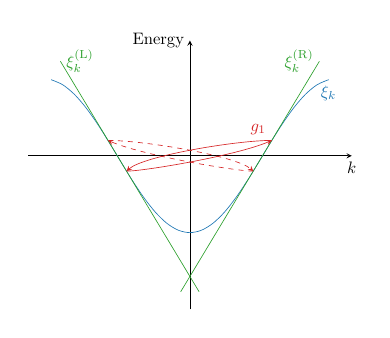
\begin{tikzpicture}[scale=0.6]
	\begin{axis}[
			axis lines=center,
			xlabel={$k$},
			ylabel={Energy},
			xlabel style={below},
			ylabel style={left},
			xtick=\empty,
			ytick=\empty,
			xmin=-3.5, xmax=3.5,
			ymin=-2.0, ymax=1.5
		]
		
		\addplot[domain=-3:3, smooth, color=tabblue]
			{-cos(deg(x))} node[below] {$\xi_k$};
		
		\addplot[domain=0.2:-2.8, color=tabgreen]
			{-1.57-x} node[right] {$\xi_k^{(\mathrm L)}$};
		
		\addplot[domain=-0.2:2.8, color=tabgreen]
			{-1.57+x} node[left] {$\xi_k^{(\mathrm R)}$};
		
		\draw[color=tabred,-stealth]
			(-1.37,-0.2) .. controls (-1,-0.2) and (1,0) .. (1.77,0.2) node[above left] {$g_1$};
		\draw[color=tabred,-stealth]
			(1.77,0.2) .. controls (1,0.2) and (-1,0) .. (-1.37,-0.2);
		
		\draw[color=tabred,dashed,-stealth]
			(1.37,-0.2) .. controls (1,-0.2) and (-1,0) .. (-1.77,0.2);
		\draw[color=tabred,dashed,-stealth]
			(-1.77,0.2) .. controls (-1,0.2) and (1,0) .. (1.37,-0.2);
		
	\end{axis}
\end{tikzpicture}
		\label{fig:g1-process}
	}
	\subfloat[][$g_2 = V(q \approx 0)$ process.]{
		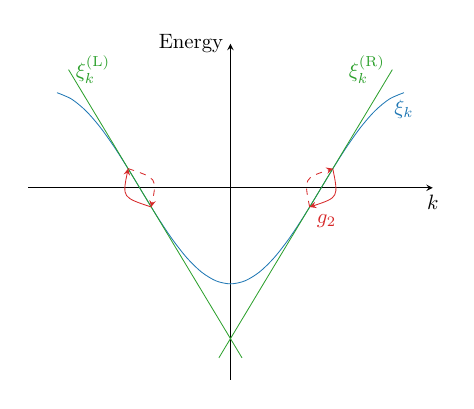
\begin{tikzpicture}[scale=0.75]
	\begin{axis}[
		axis lines=center,
		xlabel={$k$},
		ylabel={Energy},
		xlabel style={below},
		ylabel style={left},
		xtick=\empty,
		ytick=\empty,
		xmin=-3.5, xmax=3.5,
		ymin=-2.0, ymax=1.5
		]
		
		\addplot[domain=-3:3, smooth, color=tabblue]
			{-cos(deg(x))} node[below] {$\xi_k$};
		
		\addplot[domain=0.2:-2.8, color=tabgreen]
			{-1.57-x} node[right] {$\xi_k^{(\mathrm L)}$};
		
		\addplot[domain=-0.2:2.8, color=tabgreen]
			{-1.57+x} node[left] {$\xi_k^{(\mathrm R)}$};
		
		\draw[color=tabred,-stealth]
			(-1.37,-0.2) .. controls (-1.87, -0.1) .. (-1.77, 0.2);
		\draw[color=tabred,-stealth]
			(1.77,0.2) .. controls (1.87, -0.1) .. (1.37, -0.2) node[below right] {$g_2$};
			
		\draw[color=tabred,dashed,-stealth]
			(-1.77,0.2) .. controls (-1.27, 0.1) .. (-1.37,-0.2);
		\draw[color=tabred,dashed,-stealth]
			(1.37,-0.2) .. controls (1.27, 0.1) .. (1.77,0.2);
		
	\end{axis}
\end{tikzpicture}
		\label{fig:g2-process}
	}
	\subfloat[][$g_4 = V(q \approx 0)$ process.]{
		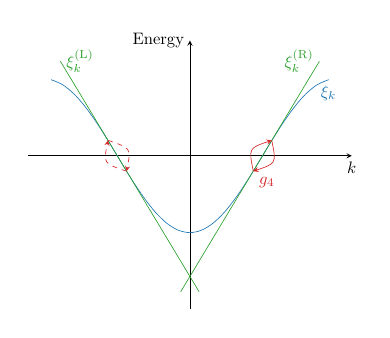
\begin{tikzpicture}[scale=0.6]
	\begin{axis}[
			axis lines=center,
			xlabel={$k$},
			ylabel={Energy},
			xlabel style={below},
			ylabel style={left},
			xtick=\empty,
			ytick=\empty,
			xmin=-3.5, xmax=3.5,
			ymin=-2.0, ymax=1.5
		]
		
		\addplot[domain=-3:3, smooth, color=tabblue]
			{-cos(deg(x))} node[below] {$\xi_k$};
		
		\addplot[domain=0.2:-2.8, color=tabgreen]
			{-1.57-x} node[right] {$\xi_k^{(\mathrm L)}$};
		
		\addplot[domain=-0.2:2.8, color=tabgreen]
			{-1.57+x} node[left] {$\xi_k^{(\mathrm R)}$};
		
		\draw[color=tabred,-stealth]
			(1.37,-0.2) .. controls (1.27, 0.1) .. (1.77, 0.2);
		\draw[color=tabred,-stealth]
			(1.77,0.2) .. controls (1.87, -0.1) .. (1.37, -0.2) node[below right] {$g_4$};
			
		\draw[color=tabred,dashed,-stealth]
			(-1.77,0.2) .. controls (-1.27, 0.1) .. (-1.37,-0.2);
		\draw[color=tabred,dashed,-stealth]
			(-1.37,-0.2) .. controls (-1.87, -0.1) .. (-1.77,0.2);
		
	\end{axis}
\end{tikzpicture}
		\label{fig:g4-process}
	}
	\caption{Diagrammatic sketch of the possible two-fermions interaction in the spinless scenario.}
	\label{fig:g-processes}
\end{figure}

It is time to let in interactions. As said, particle-hole excitations exchange a fermion from the Fermi sea with a hole from outside. Due to the strict topology of the Fermi surface, only three processes actually contribute -- namely $g_1$, $g_2$ and $g_4$, respectively in Figs.~\ref{fig:g1-process}-\ref{fig:g2-process}-\ref{fig:g4-process}. Note that, for spinless fermions, due to particles indistinguishability, actually $g_1$ and $g_2$ are the same process\footnote{
	I here skip an explanation about how to absorb $g_1$ inside $g_2$, a detail that will become clear in the spinful case.
}.

Now, consider a particle-hole symmetric interaction, \textit{quartic} in the fermionic operators,
\[
	V \sim c^\dagger c^\dagger c c
\]
as is for instance an $s$-wise spatial density-density interaction,
\[
	\hat V = \sum_{s_1 \in \left\{\mathrm L, \mathrm R\right\}} \sum_{s_2 \in \left\{\mathrm L, \mathrm R\right\}} \int_0^L dx_1 \int_0^L dx_2 \, V_{s_1 s_2}(x_1-x_2) \hat \rho_{s_1}(x_1) \hat \rho_{s_2} (x_2)
\]
coupling left-going and right-going fermions. I collect $g_4$ processes as those terms with $s_1 = s_2$ and $g_1$, $g_2$ processes as those terms with $s_1 \neq s_2$,
\[
	\underbrace{\hat \rho_\mathrm{R} (x_1) \hat \rho_\mathrm{R} (x_2) \quad \hat \rho_\mathrm{L} (x_1) \hat \rho_\mathrm{L} (x_2)}_{g_4} \qquad \underbrace{\hat \rho_\mathrm{R} (x_1) \hat \rho_\mathrm{L} (x_2) \quad \hat \rho_\mathrm{L} (x_1) \hat \rho_\mathrm{R} (x_2)}_{g_1 = g_2}
\]
At this point, I make an apparently heavy assumption I will heal later. Let me use for now a contact-like interaction,
\[
	\left[V(x-y)\right] = \frac{1}{2} \begin{bmatrix}
		g_4 & g_2 \\ g_2 & g_4
	\end{bmatrix} \delta(x-y)
	\qquad
	\text{with $g_2, g_4 \in \mathbb{R}$}
\]
(with a little notation abuse, I used the side indices $s_1$, $s_2$ as row-column indices) and let me analyze separately the contributions to the hamiltonian: $\hat V = \hat V_2 + \hat V_4$.

\paragraph{$g_4$ process.} this is the simpler case. The densities vertex contributions to $\hat K_0$ is simply
\[
	\hat V_4 = \frac{1}{2} g_4 \int_0^L dx \, \left[ \hat \rho_\mathrm{R} (x) \hat \rho_\mathrm{R} (x) + \hat \rho_\mathrm{L} (x) \hat \rho_\mathrm{L} (x) \right]
\]
Recalling Eq.~\eqref{eq:fields-density-equations},
\[
\begin{aligned}
	\hat V_4 &= g_4 \int_0^L dx \, \left[ \left( \frac{\nabla \hat \phi(x) - \nabla \hat \theta(x)}{2\pi} \right)^2 + \left( \frac{\nabla \hat \phi(x) + \nabla \hat \theta(x)}{2\pi} \right)^2 \right] \\
	&= \frac{g_4}{2\pi v_F} \times \frac{1}{2\pi} \int_0^L dx \, v_F \left[ \left( \nabla \hat \phi(x) \right)^2 + \left( \nabla \hat \theta(x) \right)^2 \right] \\
	&= \frac{g_4}{2\pi v_F} \hat K_0
\end{aligned}
\]
which is remarkable: considering this process, the hamiltonian looks like:
\[
	\hat K_0 + \hat V_4 + \hat V_2 = \frac{1}{2\pi} \int_0^L dx \, \underbrace{v_F \left( 1 + \frac{g_4}{2\pi v_F} \right)}_{u} \left[ \left( \nabla \hat \phi(x) \right)^2 + \left( \nabla \hat \theta(x) \right)^2 \right] + \hat V_2
\]
Now, $u$ is the \textbf{bosons velocity renormalized by $g_4$-like interactions}.

\paragraph{$g_2$ process.} In a very similar fashion, it is easy to obtain
\[
\begin{aligned}
	\hat V_2 &= \frac{1}{2} g_2 \int_0^L dx \, \left[ 2 \left( \frac{\nabla \hat \phi(x) - \nabla \hat \theta(x)}{2\pi} \right) \left( \frac{\nabla \hat \phi(x) + \nabla \hat \theta(x)}{2\pi} \right) \right] \\
	&= \frac{g_2}{2\pi v_F} \cdot \frac{1}{2\pi} \int_0^L dx \, v_F \left[ \left( \nabla \hat \phi(x) \right)^2 - \left( \nabla \hat \theta(x) \right)^2 \right]
\end{aligned}
\]
It is not so immediate to insert this term in the interacting hamiltonian. However, an elegant formulation exists involving two parameters $u$ and $K$:
\begin{equation}\label{eq:interacting-fields-hamiltonian}
	\hat K_0 + \hat V_4 + \hat V_2 = \frac{1}{2\pi} \int_0^L dx \, \left[ \frac{u}{K} \left( \nabla \hat \phi(x) \right)^2 + uK \left( \nabla \hat \theta(x) \right)^2 \right]
\end{equation}
trivially defined as
\[
	\frac{u}{K} \equiv 1 + \frac{g_4}{2\pi v_F} + \frac{g_2}{2\pi v_F}
	\qquad
	uK \equiv 1 + \frac{g_4}{2\pi v_F} - \frac{g_2}{2\pi v_F}
\]
a condition simultaneously satisfied by
\[
	u = v_F \sqrt{\left(1 + \frac{y_4}{2}\right)^2 - \left(\frac{y_2}{2}\right)^2}
	\qquad
	K = \sqrt{\frac{2 + y_4 - y_2}{2 + y_4 + y_2}}
	\qquad
	y_i \equiv \frac{g_i}{\pi v_F}
\]
This collection of equation is all I need to completely map a one-dimensional interacting fermionic problem into a renormalized free bosonic problem. Everything I have done hold for spinless fermions and contact interaction, but can be extended.

\subsubsection{The euclidean action}

I here briefly sketch the derivation of the bosonized euclidean action. Starting from the hamiltonian density,
\[
	\hat{\mathcal{K}}[\phi, \Pi] = \frac{1}{2\pi} \left[
			\frac{u}{K} \left( \nabla \hat \phi(x) \right)^2 + uK \left( \pi \hat \Pi(x) \right)^2
	\right]
\]
the euclidean action is immediately recovered by Legendre-transforming $\hat{\mathcal{K}}$ in imaginary time,
\[
	\begin{aligned}
		\mathcal{L}[\phi, \Pi] &= i \Pi \pdv{\tau} \phi - \mathcal{K} [\phi, \Pi] \\
		&= \frac{1}{2\pi} \left[
			2i \nabla \theta \pdv{\tau} \phi
			- \frac{u}{K} \left( \nabla \phi \right)^2 + uK \left( \nabla \theta \right)^2
		\right]
	\end{aligned}
\]
Now the calculation gets a little intricate, and I will skip it. The key point is to recognize that, being $L$ the lagrangian,
\[
	S[\phi, \Pi] \equiv \int_0^\beta d\tau \, L[\phi, \Pi] = \int_0^\beta d\tau \int_0^L dx \,  \mathcal{L}[\phi, \Pi]
\]
and $\mathcal{Z}$ the partition function
\[
	\mathcal{Z} \equiv \int \mathcal{D}[\phi] \mathcal{D}[\Pi] e^{-S[\phi, \Pi] /\hbar}
\]
one is able to complete the square for the $\nabla \theta$ part appearing in $\mathcal{L}$ and reduce the $\Pi$ part of the above integral to a gaussian form. The same trick holds for any $\Pi$-independent observable we may want to average. The final, effective $\phi$-action is just
\begin{equation}\label{eq:phi-action}
	S_\phi \equiv \frac{1}{2\pi} \int_0^\beta d\tau \int_0^L dx \, \left[
		\frac{1}{uK} \left(
			\vphantom{A^A}
			\partial_\tau \phi(x,\tau)
		\right)^2 + \frac{u}{K} \left(
			\vphantom{A^A}
			\nabla \phi(x,\tau) 
		\right)^2
	\right]
\end{equation}
which, exponentiated, is the path integral statistical weight.

\subsubsection{Spinless fermions observables}

The big, heavy (but wondrous) theoretical part is over: let's get operative. My aim is to estimate the renormalized parameters $u$ and $K$. First, it must be understood how to get them out of some observables.

\paragraph{Charge compressibility.}

A very simple observable, usable for estimating easily the ratio $u/K$, is charge compressibility. Let $\mu$ be the chemical potential,
\[
	\hat K \to \hat K - \mu \int_0^L dx \, \hat \rho(x)
\]
Following the convention of \citeauthor{giamarchi2003quantum}, I will define compressibility as
\[
	\kappa \equiv \pdv{\rho}{\mu}
	\qquad
	\rho = \frac{1}{L} \int_0^L dx \, \ev{\hat \rho(x)}
\]
(notice that usually the definition above is completed by a prefactor $\rho^{-2}$, I omit). Using Eq.~\eqref{eq:fields-density-equations}\footnote{
	To be complete, I here am hiding a passage. In fact, $\pi \hat \rho = \pi \left[ \mathrm{RR} + \mathrm{LL} + \mathrm{RL} + \mathrm{LR} \right]$ (here I use the shorthand notation $\mathrm{s}_1 \mathrm{s}_2 = \hat \psi_{s_1}^\dagger \hat \psi_{s_2}$). Taking the average value, $\pi \ev{\hat \rho} = \pi \ev{ \mathrm{RR} + \mathrm{LL}} + \pi \ev{\mathrm{RL} + \mathrm{LR}}$, and it's evident by symmetry that $\ev{\mathrm{RL} + \mathrm{LR}} = 0$; which justifies the last line, since $\pi \ev{ \mathrm{RR} + \mathrm{LL}} = - \langle \nabla \hat \phi \rangle$.
},
\[
\begin{aligned}
	\pdv{\rho}{\mu} &= \pdv{}{\mu} \frac{1}{L} \int_0^L dx \, \ev{\hat \rho(x)} \\
	&= - \frac{1}{\pi L} \pdv{}{\mu} \int_0^L dx \, \ev{\nabla \hat \phi(x)}
\end{aligned}
\]

Now, consider the term I am adding to the hamiltonian: let me add a pure energy shift term (physically irrelevant) and manipulate the above expression a bit,
\[
\begin{aligned}
	- \mu \int_0^L dx \, \hat \rho(x) &= \frac{\mu}{\pi} \int_0^L dx \, \nabla \hat \phi(x) + \Delta \\
	&= \frac{1}{2\pi} \times 2 \int_0^L dx \, \frac{u}{K} \left( \mu \frac{K}{u} \right) \left( \nabla \hat \phi(x) \right) + \underbrace{
		\frac{1}{2\pi} \int_0^L dx \, \left( \mu \frac{K}{u} \right)^2
	}_{\Delta} \\
\end{aligned}	
\]
It is now immediate to see that if I define
\[
	\hat \varphi(x) \equiv \hat \phi(x) + \mu \frac{K}{u} x
\]
we have:
\[
	\hat K - \mu \int_0^L dx \, \hat \rho(x) =  \frac{1}{2\pi} \int_0^L dx \, \left[ \frac{u}{K} \left( \vphantom{\hat\theta} \nabla \hat \varphi(x) \right)^2 + uK \left( \nabla \hat \theta(x) \right)^2 \right]
\]
an expression canonically equivalent to Eq.~\eqref{eq:interacting-fields-hamiltonian}. Now, for this new system the term $\nabla \hat \varphi$ represents charge density fluctuations. This implies that $\ev{\nabla \hat \varphi} = 0$ at any point. Then,
\[
	- \ev{\nabla \hat \phi(x)} = \mu \frac{K}{u}
\]
Finally:
\[
\begin{aligned}
	\pdv{\rho}{\mu}	&= - \frac{1}{\pi L} \pdv{}{\mu} \int_0^L dx \, \ev{\nabla \hat \phi(x)} \\
	&= \pdv{}{\mu} \mu \frac{K}{\pi u} \times \frac{1}{L} \int_0^L dx = \frac{K}{\pi u}
\end{aligned}
\]
Then, to measure the ratio $u/K$ I need to measure the quantity $(\pi \Delta \rho / \Delta \mu)^{-1}$ (times $\hbar$, to be dimensionally correct). This most certainly is a simple quantity to be measured by the means of a DMRG simulation.

\paragraph{Charge stiffness}

\begin{figure}
	\centering
	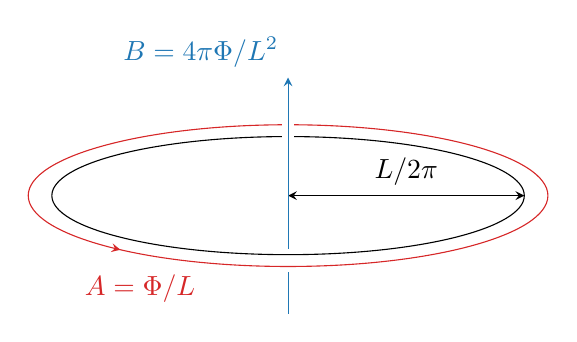
\begin{tikzpicture}[
	scale=1.5,
	decoration={
		markings,
		mark=at position 0.6 with {\arrow{stealth}}}
	]
	
	\draw[color=black, stealth-stealth]
		(0,0) -- (2,0) node[anchor=south, midway]
			{$L/2\pi$};
	\draw[color=black]
		(0,0) ellipse (2 and 0.5);
	\draw[color=tabred, postaction={decorate}] 
		(0,0) ellipse (2.2 and 0.6) node[anchor=north east, yshift=-25, xshift=-30]
			{$\displaystyle A = \Phi/L$};
	\fill[color=white]
		(-0.05, 0.45) rectangle (0.05, 0.65);
	\draw[color=tabblue, -stealth] 
		(0,-0.45) -- (0,1) node[anchor=south east]
			{$\displaystyle B = 4\pi \Phi/L^2$};
	\draw[color=tabblue]
		(0,-0.65) -- (0,-1);
\end{tikzpicture}
	\caption{Schematics of a static flux $\Phi$ pinning through a ring of circumference $L$.}
	\label{fig:flux-through-ring}
\end{figure}

Another observable rather easy to compute numerically is the charge stiffness; which is basically the tendency of the system to respond to an external charge-coupling field. Now, assuming a closed-chain topology (as in Fig.~\ref{fig:flux-through-ring}), a flux $\Phi$ threading the ring accounts for a static vector potential
\[
	A = \frac{\Phi}{L}
\]
I define the unit flux as:	$\Phi_0 \equiv h/e$. The overall effect on the fermionic system is an overall momentum shift originated by the covariant derivative formulation,
\[
	k \to k - \frac{e}{\hbar} A = k - \frac{2\pi}{L} \frac{\Phi}{\Phi_0}
\]
Let me define the shift angle:
\[
	\eta \equiv 2\pi \frac{\Phi}{\Phi_0}
\]
Finally, absorbing the latter as a gauge transformation, this translates in the presence of twisted boundary conditions by an angle $2\pi \Phi/\Phi_0$ in the wavefunction. Now, given the band $\xi_k[\Phi]$, the current density is simply
\[
	\begin{aligned}
		J &= \frac{1}{L} \sum_{k \colon \xi_k \le 0} \frac{1}{\hbar} \pdv{}{k} \xi_k[\Phi] \bigg|_\Phi \\
		&= J_0 +  \frac{1}{L\hbar} \sum_{k \colon \xi_k \le 0} L \pdv{}{\eta} \xi_k[\Phi] \bigg|_\Phi \\
		&= \frac{1}{\hbar} \pdv{\eta} E[\Phi]
	\end{aligned}
\]
In the second passage I have isolated the contribution to the derivative given from the free system $J_0$, null by symmetry, and in the last the ground-state energy $E[\Phi]$ was recognized as the sum of all single-particle occupied states.

Now, charge stiffness is simply the zero-flux current response:
\[
	\mathcal{D} = \pdv{J}{\Phi} \bigg|_{\Phi=0}
\]
As for the compressibility, I adopt a slightly different (and charge-neutral) definition,
\begin{equation}\label{eq:charge-stiffness-definition}
	\mathcal{D} \equiv \frac{\pi L}{e} \pdv{J}{\Phi} \bigg|_{\Phi=0}
\end{equation}
Inserting the previous result,
\[
	\mathcal{D} = \frac{\pi L}{e} \frac{\Phi_0}{2\pi} \pdv{J}{\eta} \bigg|_{\Phi=0} = \pi L \pdv[2]{\eta} E[\Phi] \bigg|_{\Phi=0}
\]
The second derivative of the ground-state energy, taken with respect to the twisting angle, is -- apart from some factors -- the charge stiffness.

I now need to link all of this with the bosonization scheme. The procedure is identical to the one carried out for the charge compressibility in last paragraph:
\begin{enumerate}
	\item Include the minimally coupled interaction in the euclidean effective action of Eq.~\eqref{eq:phi-action},
	\[
		S_\phi \to S_\phi - \int dx \, J(x) A(x) = S_\phi - \frac{\Phi}{L} \int dx \, J(x)
	\]
	\item The charge density current is one dimension is obtained easily from the continuity equation:
	\[
		\partial_t \rho + \nabla j = 0
		\qquad\implies\qquad
		j = \frac{1}{\pi} \partial_t \phi
	\]
	having used $\rho = - \nabla \phi/\pi$ and ignored boundary terms.
	\item A constant added to the action does not change its variational properties. Thus, defining
	\[
		\varphi \equiv \phi - uK \frac{\Phi}{L} \tau
	\]
	neither the time nor the spatial part get affected by the transformation, and the action for a flux-free system is recovered.
	\item Since for the flux-free system the induced current is zero,
	\[
		J = \frac{1}{\pi} \ev{\partial_\tau \phi} = uK \frac{\Phi}{\pi L}
	\]
\end{enumerate}
Recalling the definition of $\mathcal{D}$ of Eq.~\eqref{eq:charge-stiffness-definition}, finally
\begin{equation}\label{eq:charge-stiffness}
	\mathcal{D} = uK
\end{equation}
which is the second relation I needed in order to determine $u$ and $K$. The entirety of this derivation could have been worked out analogously by expressing the current in terms of the conjugate momentum field $\Pi$ and completing the square directly in the hamiltonian.

\paragraph{Equal-time Green's function.}

The single-particle Green's function is defined in imaginary time, and for $s$-side fermions, as:
\[
	\mathcal{G}_s (x,\tau) \equiv - \ev{\mathrm{T}_\tau \left\{ \hat \psi_s (x,\tau) \hat \psi_s ^\dagger (0,0) \right\}}
\]
having we assumed in definition spacetime translational invariance, and being $\mathcal{T}_\tau$ the time-ordering operator. Let me take $\tau = 0^-$, thus keeping the order $\hat \psi \hat \psi^\dagger$ inside the expectation value. I (surprisingly) follow here the lead of \cite{giamarchi2003quantum, senechal1999introduction}: the occupation factor $n(k)$,
\[
	n(k) \equiv \ev{\hat c_k^\dagger \hat c_k}
\]
is given by the Fourier transform of the equal time Green's function:
\[
	n(k) = \int_0^L dx \, e^{-ikx} \mathcal{G}_s (x,0^-)
\]
both for $s=\mathrm{R}, \mathrm{L}$ due to inversion symmetry. At zero temperature, the following algebraic dependence holds:
\[
	n(k) = n(k_F) - A \times \sgn(k-k_F) \abs{k-k_F}^\zeta
	\qquad
	\zeta \equiv \frac{1}{4} \left( K + \frac{1}{K} - 2 \right)
\]
with $A \in \mathbb{R}$. Then, a suitable way to extract the $K$ parameter on a lattice model simulation would be to perform the following computation:
\[
	n(k) \simeq \ev{ \mathrm{FT} \left\{ \hat c_j^\dagger \hat c_j \right\} } = \frac{1}{\sqrt{L}} \sum_{j=1}^L \ev{ \hat c_j^\dagger \hat c_j } e^{i k j}
\]
From this measure $\zeta$ can be extracted for $k<k_F$ and $k>k_F$, and from the latter $K$.

\paragraph{Equal-time density-density correlations.}

A very important feature of the bosonization scheme is the possibility of computing first-order analytical expressions for the correlations of observables. Take density-density correlations,
\[
	\mathcal{C}_\mathrm{CDW}(s) = \ev{\hat \rho(s) \hat \rho(0)}
	\quad\text{for}\quad
	s = (x,u\tau)
\]
To treat this expression in a field-theoretical fashion, I express the density operator as
\[
	\begin{aligned}
		\hat \rho(s) &= \left[
			\hat \psi_\mathrm{R}(s) + \hat \psi_\mathrm{L}(s)
		\right] \left[
			\hat \psi_\mathrm{R}(s) + \hat \psi_\mathrm{L}(s)
		\right] \\
		&= - \frac{1}{\pi} \nabla \hat \phi(s) + \left[
			\hat \psi_\mathrm{R}(s) \hat \psi_\mathrm{L}(s) + \hat \psi_\mathrm{L}(s) \hat \psi_\mathrm{R}(s) 
		\right] \\
		&= - \frac{1}{\pi} \nabla \hat \phi(s) + \frac{1}{2\pi\alpha} \left[
			e^{i 2k_F x} e^{-i 2 \hat \phi(s)}
			+ \mathrm{h.c.}
		\right]
	\end{aligned}
\]
Recall, $\alpha$ is a cutoff I introduced to stabilize the theory. In particular, $\alpha$ has the dimensions of a length and the momentum integral is cut at momenta larger than $1/\alpha$. I avoid entering in the detailed derivation: what is important, is that we can safely assume $\alpha \to 0$, at least for this correlation function \cite{haldane1981luttinger}. Let $y_\alpha$ be
\[
	y_\alpha \equiv u\tau + \alpha \sgn(\tau)
\]
The dominant behavior for $\mathcal{C}_\mathrm{CDW}(s)$ is given by
\[
	\mathcal{C}_\mathrm{CDW}(s) \simeq \frac{K}{2\pi^2} \frac{y_\alpha^2 - x^2}{(x^2 + y_\alpha^2)^2} + \frac{2}{(2\pi\alpha)^2} \cos\left(2k_F x\right) \left(
		\frac{\alpha}{\sqrt{x^2 + (u\tau)^2}}
	\right)^{2K}
	\quad\text{for}\quad \sqrt{x^2 + (u\tau)^2} \gg \alpha
\]
which, for equal-time measurement ($\tau=0$) reduces to
\begin{equation}\label{eq:density-density-correlation-power-law}
	\mathcal{C}_\mathrm{CDW}(x) \simeq - \frac{K}{2\pi^2 x^2} +  \frac{2}{(2\pi\alpha)^2} \cos\left(2k_F x\right) \left(
		\frac{\alpha}{x}
	\right)^{2K}
\end{equation}
As \citeauthor{giamarchi2003quantum} notes \cite[Sec.~2.2.2]{giamarchi2003quantum}, the first term reproduces a standard Fermi liquid correlation, decaying as $x^{-2}$ with an amplitude renormalized by interactions. The second term is highly unusual and has two remarkable properties: an amplitude modulation of wavevector $2k_F$ (a property also present in Fermi liquids, signaling the presence of a Fermi sea underneath the interactions) \textit{plus} a power-law decay whose strength is determined by interactions.

Finally, notice that for a $1$D lattice of lattice spacing $a$ at half-filling, the Fermi wavevector is given by $k_F = \pi/2a$. Since each site coordinate is $x_r=ra$, one has
\[
	\mathcal{C}_\mathrm{CDW}(r) \simeq - \frac{K}{2\pi^2 (ra)^2} +  \frac{2 (-1)^r }{(2\pi\alpha)^2} \left(
	\frac{\alpha}{ra}
	\right)^{2K}
	\quad\text{for}\quad
	r \in \mathbb{Z} \mod L
\]
The oscillatory character of the correlation function with the site index parity reflects the fact that, at half-filling, charge-density waves (CDW) excitations follow have wavelength twice the lattice spacing. At unitary filling, such oscillatory behavior vanishes due to the halving of the Fermi wavevector.

\paragraph{Superconducting correlations.}

\todo

\clearpage
\section{The Fermi-Hubbard model}

\begin{figure}
	\centering
	\subfloat[Lattice with null flux.]{
		\begin{tikzpicture}
	\foreach \i in {0,1,...,7}{
		\def\angle{45*\i}
		
		\draw[color=tabgreen]
			(\angle:2) -- ({\angle+45}:2);
			
		\node[anchor=center, color=tabgreen]
			at ({\angle+22.5}:2.2) {$t$};
		
		\filldraw[color=black]
			(\angle:2) circle (1pt);
	}
	
	\filldraw[color=black]
		(0:2) circle (1pt);
\end{tikzpicture}
		\label{subfig:lattice-ring}
	}
	\hfil
	\subfloat[Lattice with finite flux $\Phi$.]{
		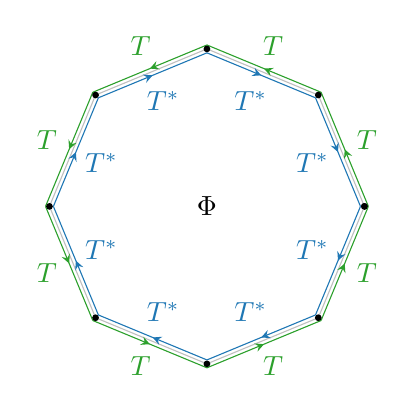
\begin{tikzpicture}[
		decoration={
		markings,
		mark=at position 0.5 with {\arrow{stealth}}}
	]
	\foreach \i in {0,1,...,7}{
		\def\angle{45*\i}
		
		\draw[color=gray!50]
			(\angle:2) -- ({\angle+45}:2);
		
		\draw[color=tabgreen, , postaction={decorate}]
			(\angle:2.05) -- ({\angle+45}:2.05);
		
		\node[anchor=center, color=tabgreen]
			at ({\angle+22.5}:2.2) {$T$};
		
		\draw[color=tabblue, , postaction={decorate}]
			({\angle+45}:1.95) -- (\angle:1.95);
		
		\node[anchor=center, color=tabblue]
			at ({\angle+22.5}:1.45) {$T^*$};
		
		\filldraw[color=black]
			(\angle:2) circle (1pt);
	}
	
	\filldraw[color=black]
	(0:2) circle (1pt);
	
	\node[anchor=center] 
		at (0,0) {$\Phi$};
\end{tikzpicture}
		\label{subfig:lattice-ring-flux}
	}
	\caption{In Fig.~\ref{subfig:lattice-ring} a schematics of a $1D$ closed lattice is portrayed. The hopping amplitude $t$ is purely real, $t = \sgn(t) \abs{t}$. In Fig.~\ref{subfig:lattice-ring-flux} the same lattice is represented, but coupled to a finite threading flux $\Phi$ which can be absorbed via the pseudo-gauge transformation in Eq.~\todo. As a consequence, the hopping amplitude acquires a chirality which manifests in a non-null imaginary part, $T = t e^{i\Phi/L}$.}
	\label{fig:lattice-rings}
\end{figure}

In this project I limit myself to a polarized (spinless fermions) system. Extension to a spinful system is possible and introduces some refinements in the general bosonization scheme, the most notable being the famous spin-charge separation. Let me take it easy: consider the following interacting hamiltonian:
\begin{equation}\label{eq:spinless-hamiltonian-pbc}
	\hat H \equiv -t \sum_{\ev{j,k}} \left[
		\hat c_j^\dagger \hat c_k + \hat c_k^\dagger \hat c_j 
	\right] + V \sum_{\ev{j,k}} \hat n_j \hat n_k - \mu \sum_{j=1}^L \hat n_j
\end{equation}
defined on a closed $1D$ lattice ring, as in Fig.~\ref{subfig:lattice-ring}.
This is a simple nearest-neighbors (NN) interacting lattice hamiltonian with NN interaction $V$, chemical potential $\mu$ and hopping amplitude $t$,
\[
	t, V, \mu \in \mathbb{R}
\]

I will also be considering a magnetic flux $\Phi$ threading the ring and coupling to the charge degree of freedom. On a ring this pinned flux acts as a tangential vector potential, which is, a momentum offset; thus the correct way to absorb into our lattice framework this interaction is via the pseudo-gauge transformation
\[
	\hat c_j \to e^{-ij \phi} \hat c_j
	\qquad\qquad
	\hat c_j^\dagger \to e^{ij \phi} \hat c_j^\dagger
	\qquad\qquad
	\phi \equiv \frac{\Phi}{L}
\]
Incorporate the latter in the above hamiltonian: the hopping amplitude becomes complex (which is, chiral) $t \to T \equiv t e^{i\phi}$, with $t, \phi \in \mathbb{R}$. We have, as in Fig.~\ref{subfig:lattice-ring-flux}
\begin{equation}\label{eq:spinless-hamiltonian-tbc}
	\hat H \equiv -t \sum_{j=1}^L \left[ 
		e^{-i\phi} \hat c_j^\dagger \hat c_{j+1} + e^{i\phi} \hat c_{j+1}^\dagger \hat c_j 
	\right] + V \sum_{j=1}^L \hat n_j \hat n_{j+1} - \mu \sum_{j=1}^L \hat n_j
\end{equation}
where a $\mod L$ operation is intended: $L+1 \leftrightarrow 1$. I want to indagate its ground-state properties. The relevant parameters will be the reduced interaction $V/t$ and chemical potential $\mu/t$.
\[
	\begin{aligned}
		V/t &> 0 \qquad
		&&\text{Repulsive interaction} \\
		V/t &< 0 \qquad
		&&\text{Attractive interaction} \\
	\end{aligned}
\]
Intuitively, if the interaction becomes dominant with respect to the hopping dynamics, the combined effect of attraction/repulsion and Pauli exclusion principle should lead to two different forms of localization. On one hand, if the interaction is strong and attractive, the ground state should be uniformly filled, because fermions save energy both by closed packing and by increasing density due to the negative chemical potential contribution ($\mu > 0$). On the other hand, a strong repulsive interaction could lead to an half-filled chain, which sacrifices the chemical potential energy gain lost by reducing the particle number by not paying the energy cost of having nearby fermions. In both cases hopping is suppressed, thus fermions are localized; now it is a matter of seeing if these states are actually realized.

\subsection{Jordan-Wigner mapping of the Heisenberg XXZ model}

\begin{figure}
	\centering
	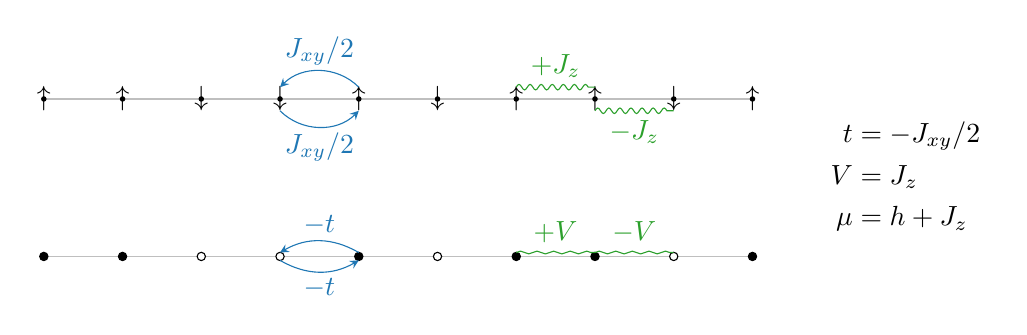
\begin{tikzpicture}
	
	% XXZ model
	\draw[color=gray!50]
		\foreach \i in {1,2,...,9}{
			(\i,0) --++ (1,0)
		};
	\fill[color=black]
		\foreach \i in {1,2,5,7,8,10}{
			(\i,0) circle (1pt) node[anchor=center]
				{$\uparrow$}
		}
		\foreach \i in {3,4,6,9}{
			(\i,0) circle (1pt) node[anchor=center]
			{$\downarrow$}
		};
	
	\draw[
		color=tabgreen,
		decorate,
		decoration={
			coil,
			aspect=0,
			amplitude=1pt,
			segment length=4pt
		}
	]
		(7,0.15) --++ (1,0) node[anchor=south, midway]
			{$+J_z$};
		
	\draw[
		color=tabgreen,
		decorate,
		decoration={
			coil,
			aspect=0,
			amplitude=1pt,
			segment length=4pt
		}
	]
		(8, -0.15) --++ (1,0) node[anchor=north, midway]
			{$-J_z$};
			
	\draw[
		color=tabblue,	
	]
		 (5,0.15) edge [-stealth, bend right=45] (4,0.15)
		 (4,-0.15) edge [-stealth, bend right=45] (5,-0.15);
		
	\node[color=tabblue, anchor=south]
		at (4.5, 0.3) {$J_{xy}/2$};
	\node[color=tabblue, anchor=north]
		at (4.5, -0.3) {$J_{xy}/2$};

	% Spinless FH model
	\draw[color=gray!50]
		\foreach \i in {1,2,...,9}{
			(\i,-2) --++ (1,0)
		};
	\filldraw[color=black, fill=black]
		\foreach \i in {1,2,5,7,8,10}{
			(\i,-2) circle (1.5pt) 
		};
	\filldraw[color=black, fill=white]
		\foreach \i in {3,4,6,9}{
			(\i,-2) circle (1.5pt)
		};
	
	\draw[
		color=tabgreen,
		decorate,
		decoration={
			coil,
			aspect=0,
			amplitude=0.5pt,
			segment length=6pt
		}
	]
		(7,-1.95) --++ (1,0) node[anchor=south, midway]
			{$+V$};
	
	\draw[
		color=tabgreen,
		decorate,
		decoration={
			coil,
			aspect=0,
			amplitude=0.5pt,
			segment length=6pt
		}
	]
		(8, -1.95) --++ (1,0) node[anchor=south, midway]
			{$-V$};
	
	\draw[
		color=tabblue,	
	]
		(5,-1.95) edge [-stealth, bend right=30] (4,-1.95)
		(4,-2.05) edge [-stealth, bend right=30] (5,-2.05);
	
	\node[color=tabblue, anchor=south]
		at (4.5, -1.85) {$-t$};
	\node[color=tabblue, anchor=north]
		at (4.5, -2.15) {$-t$};
	
	\node[align=left] 
		at (12, -1) {
			$\displaystyle
			\begin{aligned}
				t &= - J_{xy}/2 \\ 
				V &= J_z \\
				\mu &= h + J_z
			\end{aligned}$
			};
\end{tikzpicture}
	\caption{Schematics of the Jordan-Wigner mapping. The above chain represents the $\mathrm{XXZ}$ model, while the chain below represents the spinless Fermi-Hubbard model. Hollow circles represent holes, filled circles represents on-site particles. In both chain the two competing processes are represented: the NN interaction and the swapping interaction.}
	\label{fig:jordan-wigner-mapping}
\end{figure}

The model presented above can be obtained rather easily through a Jordan-Wigner of the Heisenberg XXZ model in transverse field,
\begin{equation}\label{eq:xxz-hamiltonian}
	\hat H_\mathrm{XXZ} \equiv \sum_{\ev{j,k}} \left[
		J_{xy} \left( 
			\hat S_j^x \hat S_k^x + \hat S_k^y \hat S_j^y
		\right) + J_z \hat S_j^z \hat S_k^z
	\right] - h \sum_{j=1}^L \hat S_j^z 
\end{equation}
The Jordan-Wigner mapping, only feasible in one dimension due to sites ordering, is given by:
\[
	\hat S_j^+ \to \hat c_j^\dagger e^{i\pi \sum_{k < j} \hat c_k^\dagger \hat c_k}
	\qquad
	\hat S_j^- \to \hat c_j e^{- i\pi \sum_{k < j} \hat c_k^\dagger \hat c_k}
	\qquad
	\hat S_j^z \to \hat n_j - \frac{\mathbb{I}}{2}
\]
It can be shown rather easily that, if the $c$-operators are canonically fermionic (which is, $\lbrace c_j, c_k^\dagger \rbrace = \delta_{jk}$) then the $3$D $\mathfrak{su}(2)$ spin algebra is preserved by this mapping. Notice the appearance of the Jordan parity operator up to site $j-1$, $\hat{\mathrm{P}}_{j-1}$, with
\[
	\hat{\mathrm{P}}_\ell = e^{i\pi \sum_{k \le \ell} \hat c_k^\dagger \hat c_k}
	\quad\to\quad
	(-1)^{\zeta_\ell}
	\qquad
	\zeta_\ell \equiv \sum_{k \le \ell} \hat n_k
\]
Essentially, the above string counts the fermions \textit{before} the site in question and gives back a factor $+1$ for even number, $-1$ for odd number. This works for open-ends chains, where the concept of \textit{before} is actually well-defined. 

Using basic algebra, it is straightforward to see:
\[
	\begin{aligned}
		S_j^+ \hat S_{j+1}^- &\to \left(
			\hat{\mathrm{P}}_{j-1} \hat c_j^\dagger
		\right) \left(
			\hat{\mathrm{P}}_j \hat c_{j+1}
		\right) = \hat c_j^\dagger \hat c_{j+1} \\
		S_j^- \hat S_{j+1}^+ &\to \left(
			\hat{\mathrm{P}}_{j-1} \hat c_j
		\right) \left(
			\hat{\mathrm{P}}_j \hat c_{j+1}^\dagger
		\right) = \hat c_{j+1}^\dagger \hat c_j \\
	\end{aligned}
\]
Indeed, the product operator $c_j^\dagger \hat{\mathrm{P}}_j$ vanishes if the site $j$ is occupied. Then site $j$ does not contribute to parity, giving $\mathrm{P}_{j-1}=\mathrm{P}_j$. Identical reasoning holds for the line below, completed by an anticommutation of Fermi operators. Let me take a $1\mathrm{D}$ spin chain with open boundary conditions (OBC). The transformation gives
\[
	\begin{aligned}
		\hat H_\mathrm{XXZ} &\equiv \sum_{j=1}^{L-1} \left[
			\frac{J_{xy}}{2} \left( 
				\hat S_j^+ \hat S_{j+1}^- + \hat S_j^- \hat S_{j+1}^+
			\right) + J_z \hat S_j^z \hat S_{j+1}^z
		\right] - h \sum_{j=1}^L \hat S_j^z \\
		&= \sum_{j=1}^{L-1} \left[
			\frac{J_{xy}}{2} \left(
				\hat c_j^\dagger \hat c_{j+1} + \hat c_{j+1}^\dagger \hat c_j
			\right) + J_z \left(
				\hat n_j - \frac{\mathbb{I}}{2}
			\right) \left(
				\hat n_{j+1} - \frac{\mathbb{I}}{2}
			\right)
		\right] - h \sum_{j=1}^L \left(
			\hat n_{j} - \frac{\mathbb{I}}{2}
		\right) \\
		&= \sum_{j=1}^{L-1} \left[
			\frac{J_{xy}}{2} \left(
				\hat c_j^\dagger \hat c_{j+1} + \hat c_{j+1}^\dagger \hat c_j
			\right) + J_z \hat n_j \hat n_{j+1}
		\right] - \sum_{j=1}^L h_j \hat n_{j}
		+ \frac{hL}{2} + \frac{J_z (L-1)}{2}
	\end{aligned}
\]
where I defined:
\[
	h_j = \begin{cases}
		h + J_z/2 &\qq{if} j=1,L \\
		h + J_z &\qq{if} 1<j<L
	\end{cases}
\]
Notice that for OBC the field term at the ends of the chain misses half the $J_z$ correction to the field, because of the missing interaction link.

Now I close the chain. This amounts to add a new interaction term,
\[
	\hat H_\mathrm{XXZ} \to \hat H_\mathrm{XXZ} + \frac{J_{xy}}{2} \left( 
		\hat S_L^+ \hat S_1^- + \hat S_L^- \hat S_1^+
	\right) + J_z \hat S_L^z \hat S_1^z
\]
Jordan-Wigner mapping requires a little more care here. Since
\[
	\begin{aligned}
		\hat S_L^+ \hat S_1^- &= \left(
			\hat{\mathrm{P}}_{L-1} \hat c_L^\dagger
		\right) \hat c_1 = \left(
			\hat{\mathrm{P}}_L \hat c_L^\dagger
		\right) \hat c_1 = (-1)^{\#_F -1} c_L^\dagger \hat c_1 \\
		\hat S_L^- \hat S_1^+ &= \left(
			\hat{\mathrm{P}}_{L-1} \hat c_L
		\right) \hat c_1^\dagger = \left(
			-\hat{\mathrm{P}}_L \hat c_L
		\right) \hat c_1^\dagger = -(-1)^{\#_F+1} c_L \hat c_1^\dagger = (-1)^{\#_F+1} \hat c_1^\dagger c_L
	\end{aligned}
\]
The first line holds because the $L$-th site must be empty, thus leaving unchanged the parity operator when extending $\mathrm{P}_{L-1} \to \mathrm{P}_L$, and simultaneously to evaluate the total chain parity after having applied $\hat c_1$ gives non-zero result only if the first site is occupied. Then, calling $\#_F$ the total number of fermions on the chain, the final parity is $\#-1$ which accounts for the first line sign prefactor. An analogous argument holds as well for the second line. We conclude that:
\begin{itemize}
	\item if the total number of fermions on the chain is \textbf{odd}, $\#_F = 2n+1$ for $n \in \mathbb{N}$, we can add the new interaction term to the hamiltonian with identical form,
	\begin{equation}\label{eq:xxz-hamiltonian-intermediate}
		\hat H_\mathrm{XXZ} = \sum_{j=1}^L \left[
			\frac{J_{xy}}{2} \left(
				\hat c_j^\dagger \hat c_{j+1} + \hat c_{j+1}^\dagger \hat c_j
			\right) + J_z \hat n_j \hat n_{j+1}
		\right] - (h+J_z) \sum_{j=1}^L \hat n_{j}
		\qquad
		\left(
			\hat c_{L+1} \equiv \hat c_1
		\right)
	\end{equation}
	I neglected an irrelevant energy shift. The PBC-$\mathrm{XXZ}$ model is mapped onto a spinless fermion system with odd number of fermions.
	\item if the total number of fermions on the chain is \textbf{even}, $\#_F = 2n+1$ for $n \in \mathbb{N}$, we can add the new interaction term to the hamiltonian closing the chain anti-periodically (or, equivalently, flipping the sign of the nearest-neighbor hopping term across the closing link),
	\[
		\hat H_\mathrm{XXZ} = \sum_{j=1}^L \left[
		\frac{J_{xy}}{2} \left(
				\hat c_j^\dagger \hat c_{j+1} + \hat c_{j+1}^\dagger \hat c_j
			\right) + J_z \hat n_j \hat n_{j+1}
		\right] - (h+J_z) \sum_{j=1}^L \hat n_{j}
		\quad
		\left(
			\hat c_{L+1} \equiv - \hat c_1
		\right)
	\]
	The APBC-$\mathrm{XXZ}$ model is mapped onto a spinless fermion system with even number of fermions.
\end{itemize}
For the sake of simplicity, I will limit this project to the first situation with an odd number of fermions. Since the PBC-$\mathrm{XXZ}$ admits for an exact Bethe-Ansatz solution, we can link the phase transitions of the two models.

Apart from a constant energy shift, the hamiltonian \eqref{eq:xxz-hamiltonian-intermediate} is \textit{de-facto} identical to the spinless model of Eq.~\eqref{eq:spinless-hamiltonian-pbc} via the mapping
\begin{equation}\label{eq:xxz-fermions-parameters-map}
	t = \frac{J_{xy}}{2}
	\qquad
	V = J_z
	\qquad
	\mu = h + J_z
\end{equation}
A schematics of this mapping\footnote{
	Note here that the \textit{exact} mapping between the two models up to this point would have been $t = - J_{xy}/2$. This sign flip is actually irrelevant for what concerns the goodness of the map: the zero-field PBC-$\mathrm{XXZ}$ phases are inverted under the canonical transformation given from sign-flipping the $xy$ spin components while leaving unchanged the $z$ one (see below). The same symmetry is implemented canonically for fermions by the fermionic-canonical transformation
	\[
	\hat c_i \to (-1)^i \hat c_i
	\]
	which is essentially a $\pi$ momentum shift. This transformation flips the hopping term sign leaving the others unchanged. Finally, this same sign problem would not have arisen if I would have chosen a slightly different but physically equivalent Jordan-Wigner mapping, connecting up-spins to holes and down-spins to particles.
} is given in Fig.~\ref{fig:jordan-wigner-mapping}.

\subsection*{Phase diagrams}

The phase diagram of the $\mathrm{XXZ}$ model is readily obtained by the means of exact methods like Bethe Ansatz. Of course, the dominant parameter is the ratio $J_z/J_{xy}$ which measures the dominant contribution to energy given by spin-spin NN interaction ($z$ term) and spin diffusion ($xy$ term). Whenever $\abs{J_z} = \abs{J_{xy}}$, the model is of the Heisenberg class.

\begin{figure}
	\centering
	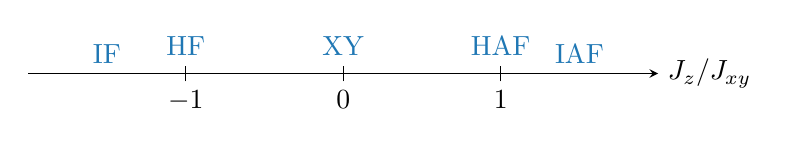
\begin{tikzpicture}[
		scale=2
	]
	\draw[color=black, -stealth]
		(-2,0) -- (2,0) node[anchor=west]
			{$J_z/J_{xy}$};
	\draw[color=black]
		(-1,-0.05) node [anchor=north] 
			{$-1$}
		-- (-1,0.05) node[anchor=south, color=tabblue] ()
			{HF}
		(0,-0.05) node [anchor=north] 
			{$0$}
		-- (0,0.05) node[anchor=south, color=tabblue]
			{XY}
		(1,-0.05) node [anchor=north] 
			{$1$} 
		-- (1,0.05) node[anchor=south, color=tabblue]
			{HAF};
		
		\node[anchor=south, color=tabblue]
			at (-1.5,0)
				{IF};
		\node[anchor=south, color=tabblue]
			at (1.5,0)
				{IAF};
\end{tikzpicture}
	\caption{Schematics for the $\mathrm{XXZ}$ model phase diagram. We are here considering a zero-field model, $h=0$ (which is mapped by the maps \eqref{eq:xxz-fermions-parameters-map} to a $\mu = J_z$ model). H indicates Heisenberg, I indicates Ising; F stands for Ferromagnet, AF for Anti-Ferromagnet; XY stands for pure $\mathrm{XY}$ model. The color of each label recalls the dominant interaction of Fig.~\ref{fig:jordan-wigner-mapping}.}
	\label{fig:xxz-phase-diagram}
\end{figure}

We can safely assume $J_{xy}>0$ and only consider the relative sign of $J_z$. This is easily seen: if we map
\[
	J_{xy} \to - J_{xy}
	\qquad
	J_z \to J_z
\]
which is, exchange the hopping sign, this is equivalent to flipping the sign of the $xy$ spin component while leaving the $z$ component unchanged. Such a map is canonical (does not impact the spin algebra). The phase diagram for negative-sign hopping is anti-symmetric with respect to this inversion. The same holds for finite field. The basic, field free phase diagram is represented schematically in Fig.~\ref{fig:xxz-phase-diagram}.
\begin{enumerate}
	\item The system tends to an Ising Ferromagnet for $J_z / J_{xy} < -1$, with dominant behavior the complete alignment of spins (which maps onto the spinless Fermi-Hubbard model as a completely filled chain). 
	\item Moving across the first Heisenberg boundary, $J_z = - J_{xy}$, the dominant behavior for energy lowering is spin diffusion up to a perfect local fields free situation of $J_z = 0$. This phase maps onto the spinless Fermi-Hubbard model as a superconducting phase.
	\item Crossing the second Heisenberg boundary, $J_z = J_{xy}$, the system tends to an Ising Anti-Ferromagnet, dominated by the Néel state configuration. The latter maps onto an half-filling and Mott-localized fermionic chain.
\end{enumerate}
For a fixed number system, this is the expected phase dynamics.

\begin{figure}
	\centering
	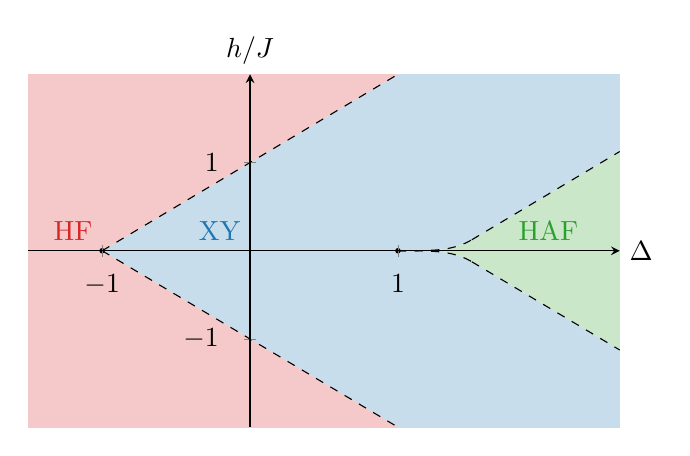
\begin{tikzpicture}
	
	\begin{axis}[
			axis lines=center,
			axis on top,
			height=0.5\textwidth,
			width=0.75\textwidth,
			xlabel={$\Delta$},		ylabel={$h/J$},
			xlabel style={right}, 	ylabel style={above},
			xtick={-1,0,1},			ytick={-1,0,1},
			xticklabel style={yshift=-0.1cm},
			yticklabel style={xshift=-0.2cm},
			xmin=-1.5, 				ymin=-2,
			xmax=2.5, 				ymax=2
		]
		
		\addplot[name path=HAFUpCurved, domain=1:1.5, dashed] 
			{2*(x-1)^4};
		\addplot[name path=HAFUpStraight, domain=1.5:2.5, dashed] 
			{x-1.375};
		\addplot[name path=HAFDownCurved, domain=1:1.5, dashed] 
			{-2*(x-1)^4};
		\addplot[name path=HAFDownStraight, domain=1.5:2.5, dashed] 
			{-x+1.375};
		\addplot[name path=HFUp1, domain=-1:1.5, dashed] 
			{x+1};
		\addplot[name path=HFUp2, domain=1.5:2.5, dashed] 
			{x+1};
		\addplot[name path=HFDown1, domain=-1:1.5, dashed] 
			{-x-1};
		\addplot[name path=HFDown2, domain=1.5:2.5, dashed] 
			{-x-1};
			
		\addplot [tabblue!25] 
			fill between [of = HAFUpCurved and HFUp1];
		\addplot [tabblue!25] 
			fill between [of = HAFUpStraight and HFUp2];
		\addplot [tabblue!25] 
			fill between [of = HAFDownCurved and HFDown1];
		\addplot [tabblue!25] 
			fill between [of = HAFDownStraight and HFDown2];
			
		\addplot[color=tabgreen!25]
			fill between [of = HAFUpCurved and HAFDownCurved];
		\addplot[color=tabgreen!25]
			fill between [of = HAFUpStraight and HAFDownStraight];
			
		\path[name path=SupportUp1] (-1.5,3) -- (-1,3);
		\path[name path=SupportUp2] (-1,3) -- (2.5,3);
		\path[name path=SupportDown1] (-1.5,-3) -- (-1,-3);
		\path[name path=SupportDown2] (-1,-3) -- (2.5,-3);
		
		\addplot[color=tabred!25]
			fill between [of = SupportUp1 and SupportDown1];
		\addplot[color=tabred!25]
			fill between [of = SupportUp1 and HFUp1];
		\addplot[color=tabred!25]
			fill between [of = SupportDown1 and HFDown1];
		
		\node[anchor=south east, color=tabblue]
			at (axis cs:0,0) {XY};
		\node[anchor=south east, color=tabred]
			at (axis cs:-1,0) {HF};
		\node[anchor=south west, color=tabgreen]
			at (axis cs:1.75,0) {HAF};
		
		\fill
			(axis cs:-1,0) circle (1pt)
			(axis cs:1,0) circle (1pt);
	
	\end{axis}
\end{tikzpicture}
	\caption{Schematics of the phase boundaries for the $\mathrm{XXZ}$ model as extracted by \citeauthor{rakov2016symmetries} \cite{rakov2016symmetries}. Notice the two zero-field phase-transition points $(-1,0)$ and $(1,0)$.}
	\label{fig:xxz-field-phase-diagram}
\end{figure}

Now, define $J$ and $\Delta$ as in \cite{rakov2016symmetries}, which is
\[
	J_{xy} \equiv J
	\qquad\qquad
	J_z \equiv J\Delta
\]
This gives the mapping:
\begin{equation}\label{eq:xxz-fermions-parameters-map-2}
	t = \frac{J}{2}
	\qquad
	\frac{V}{t} = 2\Delta
	\qquad
	\frac{\mu}{t} = 2 \left(
		\frac{h}{J} + \Delta
	\right)
\end{equation}
Within this parametrization, the analytical phase diagram is the one depicted in Fig.~\ref{fig:xxz-field-phase-diagram} \cite{rakov2016symmetries}.
Now, I use $\mu/t > 0$. This maps on the $\mathrm{XXZ}$ model as $h/J > -\Delta$, a condition depicted in Fig.~\ref{fig:jordan-wigner-mapping}. Thus, running simulations in a regime $\mu/t > 0$ and $V/t \in \mathbb{R}$, what one expects is to encounter all three phases. Now, I need to reconnect this expectation in a bosonization framework.

\begin{figure}
	\centering
	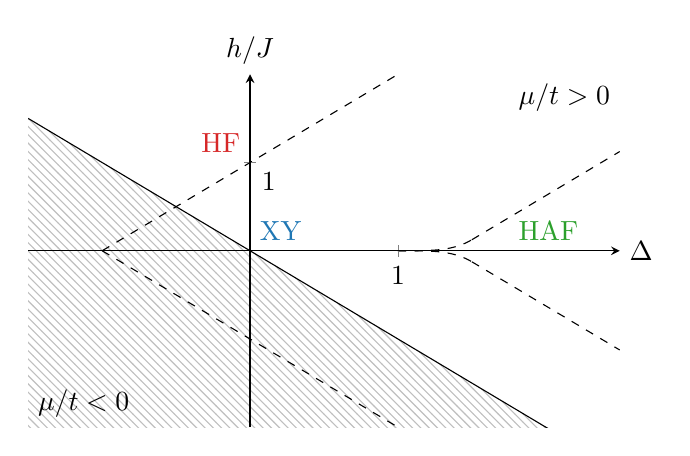
\begin{tikzpicture}
	
	\begin{axis}[
			axis lines=center,
			axis on top,
			height=0.5\textwidth,
			width=0.75\textwidth,
			xlabel={$\Delta$},		ylabel={$h/J$},
			xlabel style={right}, 	ylabel style={above},
			xtick={1},				ytick={1},
			xticklabel style={below},
			yticklabel style={below right, xshift=0.1cm},
			xmin=-1.5, 				ymin=-2,
			xmax=2.5, 				ymax=2
		]
		\addplot[name path=HAFUpCurved, domain=1:1.5, dashed] 
			{2*(x-1)^4};
		\addplot[name path=HAFUpStraight, domain=1.5:2.5, dashed] 
			{x-1.375};
		\addplot[name path=HAFDownCurved, domain=1:1.5, dashed] 
			{-2*(x-1)^4};
		\addplot[name path=HAFDownStraight, domain=1.5:2.5, dashed] 
			{-x+1.375};
		\addplot[name path=HFUp1, domain=-1:1.5, dashed] 
			{x+1};
		\addplot[name path=HFUp2, domain=1.5:2.5, dashed] 
			{x+1};
		\addplot[name path=HFDown1, domain=-1:1.5, dashed] 
			{-x-1};
		\addplot[name path=HFDown2, domain=1.5:2.5, dashed] 
			{-x-1};
		\addplot[name path=Border, domain=-1.5:2.5]
			{-x};
		\path[name path=SupportDown] 
			(-1.5,-3) -- (2.5,-3);
		\addplot[pattern=north west lines, pattern color=gray!50]
			fill between [of = SupportDown and Border];

		\node[anchor=south west, color=tabblue]
			at (axis cs:0,0) {XY};
		\node[anchor=south east, color=tabred]
			at (axis cs:0,1) {HF};
		\node[anchor=south west, color=tabgreen]
			at (axis cs:1.75,0) {HAF};
		\node[anchor=north east] 
			at (axis cs:2.5,2) {$\mu/t > 0$};
		\node[anchor=south west] 
			at (axis cs:-1.5,-2) {$\mu/t < 0$};

	\end{axis}
\end{tikzpicture}
	\caption{The same phase diagram as in Fig.~\ref{fig:xxz-field-phase-diagram}, completed with the requirement $h/J < \Delta$. The shaded area is excluded from the mapping. Note that a positive chemical potential excludes the Antiferromagnetic phase.}
	\label{fig:jordan-wigner-phase-diagram}
\end{figure}

\subsection{Non-interacting ground-state}

In order to further explore the interacting system, we need to know its zero-field non-interacting ground-state. This amounts to setting $V=\mu=0$. The hamiltonian is well known,
\[
	\hat H_0 = -t \sum_{j=1}^{L} \left(
		\hat c_j^\dagger \hat c_{j+1} + \hat c_{j+1}^\dagger \hat c_j
	\right)
\]
and is easily solved by a simple Fourier transformation,
\[
	\hat c_j \equiv \sum_k e^{ikj} \hat c_k
\]
(I am here using adimensional momenta $k$, since space has throughout been considered as a simple integer index) which leads to
\begin{equation}\label{eq:XY-hamiltonian}
	\hat H_0 = -t \sum_k \left[
		e^{-ik} \hat c_k^\dagger \hat c_k + e^{ik} \hat c_k^\dagger \hat c_k
	\right] = \sum_k \epsilon_k \hat c_k^\dagger \hat c_k
	\quad\text{for}\quad
	\epsilon_k = -2t \cos k
\end{equation}
The band $\epsilon_k$ is represented in Fig.~\ref{fig:XY-band}. At half-filling, this simple sinusoidal band presents a null Fermi energy at Fermi wavevector $k_F = \pm \pi/2$. Linearization of the band for subsequent bosonization is as well represented in Fig.~\ref{fig:XY-band}.

\begin{figure}
	\centering
	\begin{tikzpicture}
	\begin{axis}[
			axis x line=center,
			axis y line=left,
			xlabel={$k$},
			ylabel={Energy},
			xlabel style={below},
			ylabel style={above},
			xtick={-pi,0,pi},
			ytick={-1,0,1},
			extra x ticks={-pi/2,pi/2},
			extra x tick labels=\empty,
			xticklabels={$-\pi$,$0$,$\pi$},
			yticklabels={$-2t$, $0$, $2t$},
			xmin=-4.0, xmax=4.0,
			ymin=-2.0, ymax=2.0
		]
		\addplot[domain=-pi:pi, smooth, color=tabblue]
			{-cos(deg(x))} node[below] {$\epsilon_k$};
		
		\addplot[domain=0.2:-pi, color=tabgreen]
			{-1.57-x} node[right] {$\epsilon_k^{(\mathrm L)}$};
		
		\addplot[domain=-0.2:pi, color=tabgreen]
			{-1.57+x} node[left] {$\epsilon_k^{(\mathrm R)}$};
	\end{axis}
\end{tikzpicture}
	\caption{Excitations band and relative linearizations for the non-interacting model ($V=0$). At half-filling the ground-state has null Fermi energy, the negative part of the band is filled and the spectrum is gapless.}
	\label{fig:XY-band}
\end{figure}

\subsection{Bosonization of the free model}

I now \textit{bosonize} the spinless Fermi-Hubbard model. Recall the processes of Fig.~\ref{fig:g-processes}: for a spinless system the only contributions to a bosonized hamiltonian is from the $g_2$ and $g_4$ processes. The non-interacting hamiltonian is very simple, and it already known how to reduce it to the form of Eq.~\eqref{eq:free-field-hamiltonian}: all is needed is to take a coherent continuum limit for the fermionic operators,
\[
	\hat c_j \to \hat \psi(x)
\]
Let me reintroduce a lattice spacing $a$ for the sake of dimensional correctness. The bosonization of an hamiltonian of the kind of Eq.~\eqref{eq:XY-hamiltonian} has been treated at the very beginning of the present report. The only step to be done is the linearization depicted in Fig.~\ref{fig:XY-band},
\[
	-2t \cos (ka) \big|_{k = \pm \frac{\pi}{2a} + q} = 2t \cos \left(
		\pm \frac{\pi}{2} + qa
	\right) \simeq \pm (a J) q
\]
I take as granted the result of Eq.~\eqref{eq:free-field-hamiltonian}, recognizing the Fermi velocity simply as
\[
	v_F = \partial_k \epsilon_k \big|_{k = k_F} = a J
\]
(As always, I omit a term $\hbar=1$).
For the sake of completeness, here I also derive the Dirac expression for the hamiltonian density of these linear dispersion fermions (which, of course, are massless). First, split the hamiltonian of Eq.~\eqref{eq:XY-hamiltonian},
\[
	\hat H_0 \simeq \hat H_0^{(\mathrm{R})} + \hat H_0^{(\mathrm{L})}
	\quad\text{with}\quad
	\hat H_0^{(s)} \equiv \sgn(s) v_F \sum_q q \left[ \hat c_k^{(s)} \right]^\dagger \hat c_k^{(s)}
\]
I take a continuum limit: with fixed $L$, I employ $a \to 0^+$. Then, transforming back to space,
\[
	\hat c_k^{(s)} = \frac{1}{\sqrt{L}} \int_0^L dx \, e^{-ikx} \hat \psi_s(x) 
\]
Recall the shifted fields $\hat \Psi_s(x)$ of Eq.~\eqref{eq:shifted-fermionic-fields-definition}. Being $q$ defined with respect to the Fermi point $k = \sgn(s) k_F$, such that $q = k - \sgn(s) k_F$,
\[
	\hat c_k^{(s)} = \frac{1}{\sqrt{L}} \int_0^L dx \, e^{-iqx} \hat \Psi_s(x)
\]
Then
\[
	H_0^{(s)} = \sgn(s) \frac{v_F}{L} \sum_q q \int_0^L dx \, e^{iqx} \hat \Psi_s^\dagger(x) \int_0^L dy \, e^{-iqy} \hat \Psi_s(y)
\]
Since
\[
	\partial_y \left[
		e^{-iqy} \hat \Psi_s(y)
	\right] = -iq e^{-iqy} \hat \Psi_s(y) + e^{-iqy} \partial_x \hat \Psi_s(y)
\]
and integrating the left-hand side one gets zero, being the chain closed with PBC,
\[
	H_0^{(s)} = -i\sgn(s) \frac{v_F}{L} \int_0^L dx \, \hat \Psi_s^\dagger(x) \int_0^L dy \, \partial_x \hat \Psi_s(y) \sum_q e^{iq(x-y)}
\]
Using the continuum limit
\[
	\frac{1}{L} \sum_q
	\quad\to\quad
	\frac{1}{2\pi} \int_\mathbb{R} dq 
\]
the $s$-side hamiltonian finally reduces to
\[
	H_0^{(s)} = -i\sgn(s) \frac{v_F}{2\pi} \int_0^L dx \, \hat \Psi_s^\dagger(x) \partial_x \hat \Psi_s(x)
\]
Then the massless chiral Dirac hamiltonian is recovered:
\begin{equation}\label{eq:massless-Dirac-hamiltonian}
	\hat H_0 = \frac{v_F}{2\pi i} \int_0^L dx \, \left[
		\hat \Psi_\mathrm{R}^\dagger(x) \partial_x \hat \Psi_\mathrm{R}(x) - \hat \Psi_\mathrm{L}^\dagger(x) \partial_x \hat \Psi_\mathrm{L}(x)
	\right]
\end{equation}
Now, all is left to do is to insert interactions in the bosonized hamiltonian and link the model parameters to the Luttinger parameters $u$ and $K$.

\subsection{Bosonization of nearest-neighbors interaction}

The interaction term is of the density-density class,
\[
	\hat V = V \sum_{j=1}^L \hat n_j \hat n_{j+1} = a^2 J\Delta \sum_{j=1}^L \frac{\hat n_j}{a} \frac{\hat n_{j+1}}{a}
\]
We identify $\hat n_j/a \to \hat \rho(x=ja)$ as the continuum density, thus giving (splitting in left/right contributions)
\begin{equation}\label{eq:interaction-hamiltonian-lattice-density}
	\hat V = a^2 J\Delta \sum_{j=1}^L \hat \rho(ja) \hat \rho\left(
		\vphantom{A^A} (j+1)a
	\right)
\end{equation}
The detailed derivation can be found in \cite[Sec.~6.1.2]{giamarchi2003quantum}. The starting point is the expansion of $\hat \rho$, carried out in terms of physical fields $\hat \psi_s$ or shifted fields $\hat \Psi_s$ as defined in Eq.~\eqref{eq:shifted-fermionic-fields-definition},
\begin{equation}\label{eq:density-operator-shifted-fermionic-fields}
	\begin{aligned}
		\hat \rho(x) &= - \frac{1}{\pi} \nabla \hat \phi(x) + \left[
			\hat \psi_\mathrm{R}^\dagger(x) \hat \psi_\mathrm{L}(x) + \hat \psi_\mathrm{L}^\dagger(x) \hat \psi_\mathrm{R}(x) 
		\right] \\
		&= - \frac{1}{\pi} \nabla \hat \phi(x) + \left[
			e^{-2ik_F x}
			\hat \Psi_\mathrm{R}^\dagger(x) \hat \Psi_\mathrm{L}(x) + e^{2ik_F x} \hat \Psi_\mathrm{L}^\dagger(x) \hat \Psi_\mathrm{R}(x) 
		\right]
	\end{aligned}
\end{equation}
In thermodynamic limit, recalling Eq.~\eqref{eq:fermionic-fields-bosonic-fields-expression},
\[
	\hat \Psi_s (x) = \frac{\hat U_s}{\sqrt{2\pi\alpha}} \exp\left\{
		i \left(
			\sgn(s) \hat \phi(x) + \hat \theta(x)
		\right)
	\right\}
	\qquad\left( \alpha \to 0 \right)
\]
The analytical calculation gets a little cumbersome: I only highlight the essential passage. First, express analytically the density operator of Eqns.~\eqref{eq:density-operator-shifted-fermionic-fields} using the results
\[
	\hat \Psi_\mathrm{R}^\dagger(x) \hat \Psi_\mathrm{L}(x) = \frac{\hat U_\mathrm{R}^\dagger \hat U_\mathrm{L}}{2\pi\alpha} e^{-2i\hat \phi(x)}
	\qquad
	\hat \Psi_\mathrm{L}^\dagger(x) \hat \Psi_\mathrm{R}(x) = \frac{\hat U_\mathrm{L}^\dagger \hat U_\mathrm{R}}{2\pi\alpha} e^{2i\hat \phi(x)}
\]
which gives
\begin{equation}\label{eq:density-operator-bosonic-fields}
	\hat \rho(x) = - \frac{1}{\pi} \nabla \hat \phi(x) + \left[
		e^{-2ik_F x}
		\frac{\hat U_\mathrm{R}^\dagger \hat U_\mathrm{L}}{2\pi\alpha} e^{-2i\hat \phi(x)}
		+ e^{2ik_F x}
		\frac{\hat U_\mathrm{L}^\dagger \hat U_\mathrm{R}}{2\pi\alpha} e^{2i\hat \phi(x)} 
	\right]
\end{equation}
Insert now the above result in Eq.~\eqref{eq:interaction-hamiltonian-lattice-density} for both the densities appearing. The key property to be used here is that the shifted fields $\hat \Psi_s$ (and hence the bosonic fields) vary \textit{slowly} with respect to $k_F$. This means that, in the limit $a \to 0$ of null lattice spacing, one can approximate the spatial variation as only happening in the fast-oscillating exponents of the above equation. This assumption limits this derivation to slight fluctuations of the fields around equilibrium, which means, to perturbative results. Moreover, one identifies the cutoff $\alpha$ with $a$, sending both to zero. The two densities multiplied in Eq.~\eqref{eq:interaction-hamiltonian-lattice-density} then give rise to $3 \times 3 = 9$ terms, of which the most relevant are
\begin{itemize}
	\item the one coming from the $\phi$ field gradients multiplied,
	\[
		\frac{1}{\pi^2} \nabla \hat \phi(x) \nabla \hat \phi(x+a) \simeq \frac{1}{\pi^2} \left( \nabla \hat \phi(x) \right)^2
	\]
	Such approximation is possible because, as said, fields vary slowly and then $x+a$ can be taken to be $x$ as well when a field variable;
	\item the one coming from the multiplication of the second term of Eq.~\eqref{eq:density-operator-bosonic-fields} (evaluated at $x$) with the third one (evaluated at $x+a$)
	\[
		e^{-2ik_F x}
		\frac{\hat U_\mathrm{R}^\dagger \hat U_\mathrm{L}}{2\pi a} e^{-2i\hat \phi(x)} \times
		e^{2ik_F (x+a)}
		\frac{\hat U_\mathrm{L}^\dagger \hat U_\mathrm{R}}{2\pi a} e^{2i\hat \phi(x+a)} = \frac{1}{(2\pi a)^2} e^{2ik_F a} e^{2i \left[ \hat \phi(x+a) - \hat \phi(x) \right]}
	\]
	where I dropped the Klein factors and substituted $\alpha \to a$;
	\item the hermitian conjugate of the above term, which arises inverting the roles in the previous point.
\end{itemize}
The other terms either vanish when summed to their respective hermitian conjugate or are subdominant\footnote{
	A word of caution fits here. Another term actually appears in the expansion, namely a \textit{umklapp} term. As is explained by \citeauthor{giamarchi2003quantum} in \cite[Sec.~6.1.2]{giamarchi2003quantum}, for a spinless hamiltonian defined on a lattice this term is less relevant when compared to the others (but is far from irrelevancy for a complete physical description!).
}. Then
\[
	\hat \rho(x) \hat \rho (x+a) \simeq \frac{1}{\pi^2} \left( \nabla \hat \phi(x) \right)^2
	+ \frac{1}{(2\pi a)^2} e^{2ik_F a} e^{2i \left[ \hat \phi(x+a) - \hat \phi(x) \right]} + \frac{1}{(2\pi a)^2} e^{-2ik_F a} e^{-2i \left[ \hat \phi(x+a) - \hat \phi(x) \right]}
\]
Finally, approximating
\[
	\begin{aligned}
		e^{\pm 2i \left[ \hat \phi(x+a) - \hat \phi(x) \right]} &\simeq e^{\pm 2ia \nabla \hat \phi(x)} \\
		&\simeq 1 \pm 2ia \nabla \hat \phi(x) - 2a^2 \left( \nabla \hat \phi(x) \right)^2
	\end{aligned}
\]
The $1$ constant term can be discarded: it only generates a constant energy shift. The linear terms $ \pm 2ia \nabla \hat \phi(x)$ can be discarded as well, since they vanish when summed. Only the last survives:
\[
	\begin{aligned}
		\hat \rho(x) \hat \rho (x+a) &\simeq \frac{1}{\pi^2} \left( \nabla \hat \phi(x) \right)^2 
		- \frac{2a^2}{(2\pi a)^2} \left( \nabla \hat \phi(x) \right)^2 \left(
			e^{2ik_F a} + e^{-2ik_F a}
		\right) \\
		&= \frac{1}{\pi^2} \left( \nabla \hat \phi(x) \right)^2 \left(
			\vphantom{A^A}
			1 - \cos(2k_F a)
		\right) \\
		\text{(at half filling)} &= \frac{2}{\pi^2} \left( \nabla \hat \phi(x) \right)^2
	\end{aligned}
\]
It's done. Recalling the bosonic structure of the general bosonized spinless Luttinger hamiltoninan of Eq.~\eqref{eq:interacting-fields-hamiltonian}, we finally conclude that the bosonized interacting hamiltonian is given by
\begin{equation}\label{eq:XXZ-luttinger-hamiltonian}
	\frac{1}{2\pi} \int_0^L dx \, \left[ \frac{u}{K} \left( \nabla \hat \phi(x) \right)^2 + uK \left( \nabla \hat \theta(x) \right)^2 \right]
	\quad\text{with}\quad
	\begin{cases}
		uK &= aJ \\
		u/K &= aJ \left(
			1 + 4\Delta/\pi
		\right)
	\end{cases}
\end{equation}
This simple result is a consequence of the many approximations I made. It is far from exact and strictly perturbative. By the means of Bethe Ansatz, a much better result can be obtained. It must be said, by the time the author got to this point, the hopes for the simulated data to be anywhere near any of these results were narrow.

\clearpage
\section{Algorithms and simulations}

This section is devoted to delineate the system properties we aim to simulate. The algorithm used is finite-size DMRG, implemented in the \href{https://docs.julialang.org/en/}{\texttt{Julia language}} via the well supported \href{https://itensor.github.io/ITensors.jl/stable/index.html}{\texttt{ITensors.jl}}, \href{https://itensor.github.io/ITensorMPS.jl/stable/}{\texttt{ITensorsMPS.jl}} packages.

\subsection{What I would have liked to do}

A good target is to extract the Bosonization parameters $u$ and $K$ for the spinless Fermi-Hubbard model of Eq.~\eqref{eq:spinless-hamiltonian-pbc}. As said in Sec.~\ref{subsubsec:spinless-fermions-observables}, for a spinless model the task can be easy enough by performing the calculation of the charge compressibility $\kappa$ and the charge stiffness $\mathcal{D}$. From Eq.~\eqref{eq:charge-compressibility} and \eqref{eq:charge-stiffness} respectively,
\begin{equation}\label{eq:charge-compressibility-stiffness-definitions}
	\kappa = \frac{K}{\pi u}
	\qquad\text{and}\qquad
	\mathcal{D} = uK
\end{equation}
which in turn implies
\begin{equation}\label{eq:u-K-formulas}
	u = \sqrt{\frac{\mathcal{D}}{\pi\kappa}}
	\qquad\text{and}\qquad
	K = \sqrt{\pi\kappa\mathcal{D}}
\end{equation}
Coherently with the definitions I used, the observables $\kappa$ and $\mathcal{D}$ were calculated as follows. Let me define:
\begin{equation}\label{eq:fixed-number-energy-definition}
	E_g \left[
		L,N,\eta;\frac{V}{t},\frac{\mu}{t}
	\right]
\end{equation}
as the ground-state energy for the model setup specified by its arguments $L$ (size), $N$ (number of particles), $\eta$ (adimensional magnetic flux) and parameters $V/t$ (reduced NN interaction) and $\mu/t$ (reduced chemical potential). From now on I omit $V/t$ and $\mu/t$ as explicit parameters. 

\paragraph{Charge compressibility.}
Charge compressibility is given by
\[
	\kappa^{-1} = L \pdv[2]{E}{N}
\]
which is well approximated at half-filling by
\begin{equation}\label{eq:charge-compressibility-approximation}
	\kappa_{1/2}(L) \equiv \left[
		\frac{E_g[L,L/2+2,0]+E_g[L,L/2-2,0]-2E_g[L,L/2,0]}{4}
	\right]^{-1}
\end{equation}
(usually one adds or removes $2$ particles in order to avoid even-odd effects). This strategy is good for mapping the compressibility in the canonical ensemble, for which the energy is minimized each time given a fixed particles number. For a mapping of compressibility over the $[V/t,\mu/t]$ evidently one needs to let the particles number vary in order to find the gran-canonical ground state. I adopted a rather rough but coherent strategy, approximated the compressibility via its finite-differences derivative formulation
\[
	\kappa \simeq \frac{\Delta \rho}{\Delta \mu} = \frac{1}{L} \frac{\Delta}{\Delta \mu} \langle \hat N \rangle
\]
where $\langle \hat N \rangle$ is the expected total particles number evaluated at two subsequent simulations with identical $V/t$ and chemical potential differing by $\Delta \mu$.

\paragraph{Charge stiffness.}
Similarly, charge stiffness is given by
\[
	\mathcal{D} = \pi L \pdv[2]{E}{\eta}
\]
which as well is approximated at half filling by
\begin{equation}\label{eq:charge-stiffness-approximation}
	\mathcal{D}_{1/2}(L) \equiv
	\frac{E_g[L,L/2,\delta\eta]+E_g[L,L/2,-\delta\eta]-2E_g[L,L/2,0]}{4(\delta\eta)^2}
\end{equation}
for a ``small'' flux variation $\delta\eta$. It is important to notice here that the charge compressibility is expected to vanish in gapped phases. The reason is simple: if $\partial_\mu \rho=0$, that means that shifting infinitesimally the chemical potential does not increase charge density -- there is no single-particle state that can accommodate additional particles. Thus, there is a gap. A simple and good signal that a phase has become gapless is the non-vanishing charge compressibility.

\subsection{What I actually did}

All I described in the above section is a rather good strategy, provided you can simulate a big long chubby chain with a lot of fermions. It turns out, taken into account my computational resources, the entire strategy turns out to be a little optimistic. It would have been wiser to understand my limits earlier, but that's how life goes, I guess.

\subsubsection*{Charge gaps}

For a model of the class of the spinless Fermi-Hubbard, Eq.~\eqref{eq:spinless-hamiltonian-pbc}, the chemical potential part amounts to a pure energy shift when working inside a fixed-number subspace of the many-body Hilbert space. Let $E_g[L,N,\eta]$ be the ground-state energy of Eq.~\eqref{eq:fixed-number-energy-definition} at fixed particle number $N$. Moreover, let me define
\[
	\Delta_\rho^{\pm M}[\mu] \equiv E_g[L, \rho L \pm M, \eta] - E_g[L, \rho L, \eta]
\]
being $\rho \equiv N/L$ the charge filling and $M \in \mathbb{N}$ a given number of particles ($+$ sign) or holes ($-$ sign) added as elementary excitations. To diagonalize the model \eqref{eq:spinless-hamiltonian-pbc} at fixed particles number means that the energy difference must depend on $\mu/t$ only by the total number of particles, while on $V/t$ in some complicated unspecified way. This implies
\[
	\Delta_\rho^{\pm M}[\mu] \equiv f\left(
		\rho, \frac{V}{t} 
	\right) \mp M \mu
	\quad\implies\quad
	f\left(
		\rho, \frac{V}{t} 
	\right) = \Delta_\rho^{\pm M}[\mu] \pm M\mu
\]
The parametric dependence of the $\Delta$s on $\mu$ was specified explicitly. The left-hand side is independent of $\mu$. Let me define $\mu_\rho^\pm$ as the chemical potential at which the gap closes -- which is, the set of points on the $[V/t,\mu/t]$ plane where to add particles or holes does not cost energy. Then, computing the above equation's right-hand side at zero chemical potential, it must be
\[
	\mu_\rho^{\pm M} = \mp \frac{1}{M} \Delta_\rho^{\pm M}[0]
\]
Now, recall the notation of Fig.~\ref{fig:expected-sfh-phase-diagram}: for the half-filling Mott insulating region, $\mathrm{MI}_{1/2}$, the top and bottom borders shall be given by
\[
	\mu_{1/2}^{\pm 1} = \mp \Delta_{1/2}^{\pm 1}[0]
	\qquad\text{and}\qquad
	\mu_{1/2}^{\pm 2} = \mp \frac{1}{2} \Delta_{1/2}^{\pm 2}[0]
\]
I reported both the expressions for $M=1$ and $M=2$: in our PBC-$\mathrm{XXZ}$ general scheme it is formally more correct to perform fixed-$N$ computations preserving the fermion number parity. For the unitary-filling region, $\mathrm{MI}_1$, of course it is not possible to add particles; as expected, just a $-$ phase boundary can be defined at unitary density
\[
	\mu_1^{-1} = -\Delta_1^{-1}[0]
	\qquad\text{and}\qquad
	\mu_1^{-2} = -\frac{1}{2} \Delta_1^{-2}[0]
\]
To compute $\Delta_\rho^{\pm M}[\mu]$ is just a matter of computing ground-state energies. This procedure allows for a simple estimation of the phase boundaries and, most importantly, provides insight on the finite-size effects.

\subsubsection*{Single-point characterization}

A good task is to characterize the three phases by choosing one precise set of parameters representative of each. Each choice $(V/t,\mu/t)$ describes a model whose solution is a given physical phase.

{\color{tabred} [Study of precise states (one for each phase): block density variance, compressibility and charge stiffness, plot of the correlation functions, bipartite entropy.]}

\subsubsection*{Observables heatmaps}
{\color{tabred} [Density heatmap and phase identification.]}

\printbibliography \nocite{*}

\end{document}
